\documentclass[twoside]{article}

\usepackage{aistats2026}
% Under submission option (leave empty without [accepted] for double-blind review notice)

\usepackage{amsmath, amssymb, amsthm}
\usepackage{mathtools}
\usepackage{natbib}
\usepackage{graphicx}
\usepackage{subcaption}
\usepackage{booktabs}
\usepackage{hyperref}
\usepackage{algorithm, algpseudocode}
\usepackage{microtype}

\newtheorem{theorem}{Theorem}
\newtheorem{lemma}[theorem]{Lemma}
\newtheorem{proposition}[theorem]{Proposition}
\newtheorem{corollary}[theorem]{Corollary}
\newtheorem{definition}{Definition}
\newtheorem{remark}{Remark}
\newtheorem{assumption}{Assumption}

\newcommand{\E}{\mathbb{E}}
\newcommand{\R}{\mathbb{R}}
\newcommand{\Pb}{\mathbb{P}}
\newcommand{\cN}{\mathcal{N}}
\newcommand{\cD}{\mathcal{D}}
\newcommand{\cH}{\mathcal{H}}
\newcommand{\cA}{\mathcal{A}}
\newcommand{\cK}{\mathcal{K}}
\newcommand{\DP}{\text{DP}}
\newcommand{\Dir}{\text{Dir}}
\newcommand{\KL}{\text{KL}}
\newcommand{\Var}{\text{Var}}

\begin{document}

\twocolumn[

\aistatstitle{On the Regret of Approximate Thompson Sampling: \\ Why Laplace Fails and How Dirichlet Process Posterior Sampling Succeeds}

\aistatsauthor{Anonymous Authors}

\aistatsaddress{Affiliation Anonymous} ]

\begin{abstract}
Thompson Sampling (TS) is a cornerstone of multi-armed bandits, but in non-conjugate likelihood settings, practitioners universally resort to approximate posterior sampling, predominantly parametric Laplace approximations. Despite widespread use, approximate TS frequently suffers catastrophic linear regret $\Omega(T)$. We provide a unified theoretical diagnosis for this failure: parametric Laplace and variational approximations enforce compact Gaussian tail decay and local curvature estimates that systematically underestimate epistemic tail uncertainty in under-explored regions, violating the anti-concentration (stochastic optimism) condition and triggering premature arm freezing. To overcome this fundamental pathology, we analyze \emph{Dirichlet Process Posterior Sampling} (DPPS) under realistic computational approximations: Monte Carlo batch subsampling of size $B_{\text{batch}}$ and finite stick-breaking truncation at level $K_{\text{prior}}$. We prove that Approximated DPPS strictly preserves anti-concentration, achieving optimal problem-dependent frequentist regret $\mathcal{O}\left(\sum_{a \ne a^\star} \frac{\log T}{\Delta_a}\right)$ with strictly $\mathcal{O}(1)$ per-step decision latency. Empirical benchmarks confirm that Approximated DPPS completely eliminates premature arm freezing while running over $7.6\times$ faster than Laplace-TS.
\end{abstract}

\section{INTRODUCTION}
\label{sec:intro}

The multi-armed bandit (MAB) problem formalizes the fundamental trade-off between exploration (acquiring information about uncertain actions) and exploitation (capitalizing on actions known to yield high rewards) \citep{lattimore2020bandit}. Among the myriad of algorithms developed to address this dilemma, \emph{Thompson Sampling} (TS) \citep{thompson1933likelihood, russo2018tutorial} has emerged as one of the most effective and widely adopted paradigms. By maintaining a posterior distribution over environment parameters and choosing actions in proportion to the probability that they are optimal, TS achieves near-optimal empirical performance alongside asymptotically optimal problem-dependent regret guarantees \citep{agrawal2012analysis, kaufmann2012thompson}.

In textbook settings with conjugate prior-likelihood pairs (such as Beta-Bernoulli or Gaussian-Gaussian models), posterior updates are closed-form, and exact Thompson Sampling is straightforward. In modern practical applications, however, reward likelihoods are routinely non-conjugate, non-Gaussian, or multimodal \citep{chapelle2011empirical, riquelme2018deep}. In such domains, exact posterior calculation is analytically intractable. 

To operationalize Thompson Sampling in these non-conjugate environments, the standard machine learning literature overwhelmingly relies on \emph{approximate inference} \citep{chapelle2011empirical, phan2019thompson, mazumdar2020approximate}. Foremost among these is the \textbf{Laplace approximation}, which fits a Gaussian distribution centered at the maximum a posteriori (MAP) estimate with covariance given by the inverse Hessian of the negative log-posterior \citep{mackay2003information, bishop2006pattern}. Laplace-TS has become a default workhorse for logistic bandits, click-through-rate prediction, and Bayesian optimization.

\paragraph{The Failure of Approximate TS.}
Despite its widespread adoption, approximate Thompson Sampling exhibits a notorious, dark failure mode: on simple, non-adversarial bandit problems, algorithms relying on Laplace approximations or variational inference (VI) frequently collapse into \textbf{linear regret $\Omega(T)$} \citep{lu2017ensemble, dwarakanath2020limitations}. While practitioners often attribute this pathology to numerical instability or optimizer tolerance, the fundamental statistical mechanism driving this collapse has remained incompletely understood.

\paragraph{Our Contributions.}
In this paper, we resolve this open theoretical problem and present a principled Bayesian nonparametric solution:
\begin{enumerate}
    \item \textbf{Theoretical Diagnosis of Laplace Failure:} We prove that the failure of Laplace-TS is caused by a structural violation of the \emph{Anti-Concentration (Stochastic Optimism)} property. When early observations accidentally underestimate the true mean of the optimal arm, the local quadratic curvature of the Laplace approximation severely underestimates epistemic tail uncertainty. The Gaussian tail drops exponentially fast, reducing the probability of sampling the optimal arm to zero and permanently freezing exploration, resulting in provable frequentist linear regret $\Omega(T)$ (Theorem~\ref{thm:laplace_failure}).
    \item \textbf{Approximated Dirichlet Process Posterior Sampling (DPPS):} We revisit the DPPS framework introduced by \citet{vashishtha2025leveraging} and further developed in \citet{vashishtha2026tmlr, vashishtha2026thesis}, which places a Dirichlet Process prior $\text{DP}(\alpha, F_0)$ directly on the reward generating distribution of each arm. To make DPPS scalable to large time horizons, we analyze it under practical, computationally bounded approximations: (i) \emph{Monte Carlo batch subsampling} of size $B_{\text{batch}}$ from the historical observation buffer, and (ii) \emph{finite stick-breaking truncation} at level $K_{\text{prior}}$.
    \item \textbf{Frequentist Regret Guarantees under Approximations:} We prove that unlike Laplace approximations, Approximated DPPS provably preserves the anti-concentration property for any time horizon $T$ (Theorem~\ref{thm:dpps_anti_concentration}). As long as the base measure $F_0$ covers the support of the rewards and $K_{\text{prior}} = \Omega(\log T)$, Approximated DPPS achieves the optimal problem-dependent frequentist regret bound $\mathcal{O}\left(\sum_{a \ne a^\star} \frac{\log T}{\Delta_a}\right)$ (Theorem~\ref{thm:dpps_regret}).
    \item \textbf{Unifying Non-Parametric Thompson Sampling (NPTS):} We prove that the celebrated NPTS algorithm of \citet{riou2020bandit} is an algebraically identical special case of DPPS with $\alpha = 1$ and a degenerate point mass base measure $F_0 = \delta_B$ at a known upper bound $B$. We show how DPPS overcomes NPTS's fatal vulnerability when the upper bound $B$ is unknown or misspecified.
    \item \textbf{Empirical Verification:} Across diverse non-conjugate, skewed, and logistic multi-armed bandit benchmarks, we demonstrate that Laplace-TS suffers severe premature arm freezing and linear regret, whereas Approximated DPPS consistently achieves logarithmic regret while operating with bounded computational cost per round.
\end{enumerate}

---

\section{PROBLEM FORMULATION \& FOUNDATIONS OF TS}
\label{sec:formulation}

We consider a stochastic Multi-Armed Bandit (MAB) with $K$ arms, indexed by $a \in \mathcal{A} = \{1, \dots, K\}$. At each discrete time step $t \in \{1, \dots, T\}$, the decision maker selects an arm $A_t \in \mathcal{A}$ and observes a reward $r_t \sim P^\star_{A_t}$, where $P^\star_a$ is an unknown, fixed probability distribution supported on $\mathcal{R} \subseteq \mathbb{R}$.

Let $\mu_a = \mathbb{E}_{r \sim P^\star_a}[r]$ denote the true expected reward of arm $a$. The optimal arm is denoted by $a^\star = \arg\max_{a \in \mathcal{A}} \mu_a$, with optimal value $\mu^\star = \mu_{a^\star}$. For each sub-optimal arm $a \ne a^\star$, the sub-optimality gap is defined as $\Delta_a = \mu^\star - \mu_a > 0$. Let $N_a(t) = \sum_{\tau=1}^t \mathbb{I}\{A_\tau = a\}$ be the number of times arm $a$ has been selected up to time $t$. The historical observation buffer for arm $a$ is $\mathcal{H}_{a, t} = \{r_{a, 1}, \dots, r_{a, N_a(t)}\}$, and the full filtration is $\mathcal{F}_t = \sigma(A_1, r_1, \dots, A_t, r_t)$.

The performance of an algorithm is evaluated via its **frequentist (problem-dependent) cumulative regret**:
\begin{equation}
R(T) = \mathbb{E}\left[ \sum_{t=1}^T (\mu^\star - \mu_{A_t}) \right] = \sum_{a: \Delta_a > 0} \Delta_a \mathbb{E}[N_a(T)],
\label{eq:frequentist_regret}
\end{equation}
where the expectation is taken solely with respect to the stochasticity of the environment rewards and the internal randomization of the policy.

\subsection{Canonical Regret Decomposition of Thompson Sampling}

In Thompson Sampling, at each time step $t$, the agent draws a posterior sample $\tilde{\mu}_a(t)$ for each arm $a \in \mathcal{A}$ from its current belief distribution $\mathcal{P}_a(\cdot \mid \mathcal{H}_{a, t-1})$, and selects the arm with the highest sampled index:
\begin{equation}
A_t = \arg\max_{a \in \mathcal{A}} \tilde{\mu}_a(t).
\label{eq:ts_rule}
\end{equation}

In canonical bandit theory \citep{agrawal2012analysis, agrawal2013further, russo2014information}, the probability of playing a sub-optimal arm $a$ is bounded by decomposing the event into whether the optimal arm $a^\star$ was under-sampled or the sub-optimal arm $a$ was over-sampled. Sublinear regret requires two complementary probabilistic properties:

\begin{definition}[Concentration of Sub-optimal Arms]
An exploration algorithm satisfies concentration if for any sub-optimal arm $a \ne a^\star$ and any deviation $\epsilon > 0$, the probability of overestimating its mean decays exponentially in sample count:
\begin{equation}
\mathbb{P}\left(\tilde{\mu}_a(t) \ge \mu_a + \epsilon \mid \mathcal{F}_{t-1}\right) \le C_1 \exp\left( - c_1 N_a(t-1) \epsilon^2 \right).
\label{eq:concentration}
\end{equation}
\end{definition}

\begin{definition}[Anti-Concentration / Stochastic Optimism]
An exploration algorithm satisfies anti-concentration (or stochastic optimism) if the sampled index of the optimal arm has a strictly non-vanishing probability of exceeding its true mean:
\begin{equation}
\mathbb{P}\left(\tilde{\mu}_{a^\star}(t) \ge \mu^\star \mid \mathcal{F}_{t-1}\right) \ge p_0 > 0 \quad \text{almost surely},
\label{eq:anti_concentration}
\end{equation}
for some positive constant $p_0 > 0$ independent of $t$.
\end{definition}

When both conditions hold, standard Thompson Sampling guarantees:
\begin{equation}
\begin{aligned}
\mathbb{E}[N_a(T)] &\le \frac{C \log T}{\Delta_a^2} + \mathcal{O}(1) \\
\implies R(T) &\le \mathcal{O}\left( \sum_{a \ne a^\star} \frac{\log T}{\Delta_a} \right).
\end{aligned}
\end{equation}

---

\section{WHY PARAMETRIC CURVATURE APPROXIMATIONS FAIL STOCHASTIC OPTIMISM}
\label{sec:laplace_failure}

In non-conjugate likelihood settings, exact posterior sampling is computationally intractable. Practitioners overwhelmingly turn to **parametric approximations**: most notably, **Laplace Gaussian approximations** around the MAP mode \citep{chapelle2011empirical, mackay2003information, phan2019thompson, mazumdar2020approximate} and **Mean-Field Variational Inference (MFVI)** \citep{bishop2006pattern, riquelme2018deep}. We now demonstrate that this entire class of parametric approximations shares a fundamental theoretical flaw: their local curvature estimates catastrophically underestimate epistemic tail uncertainty in under-sampled regions, violating anti-concentration and triggering premature arm freezing. We examine the Laplace approximation as the canonical, analytically transparent exemplar.

Consider a non-conjugate setting, such as a **Logistic Bernoulli Bandit** \citep{chapelle2011empirical}, where rewards $r \in \{0, 1\}$ are parameterized by an unknown latent logit parameter $\theta_a \in \mathbb{R}$:
\begin{equation}
\mathbb{P}(r = 1 \mid \theta_a) = \sigma(\theta_a) = \frac{1}{1 + e^{-\theta_a}}, \quad \mu_a = \sigma(\theta_a^\star).
\end{equation}
A prior $\theta_a \sim \mathcal{N}(0, \sigma_0^2)$ is placed on the latent parameters. Given $n = N_a(t-1)$ observations with $s = \sum_{i=1}^n r_i$ successes, the true posterior density is:
\begin{equation}
p(\theta_a \mid \mathcal{H}_{a, t-1}) \propto \exp\left( s \theta_a - n \log(1 + e^{\theta_a}) - \frac{\theta_a^2}{2\sigma_0^2} \right).
\end{equation}
Because the normalizer is analytically intractable, the **Laplace approximation** approximates this posterior by a Gaussian centered at the MAP estimate $\hat{\theta}_a$:
\begin{equation}
q_t(\theta_a) = \mathcal{N}\left( \hat{\theta}_a, \; \sigma_{\text{Lap}, a}^2 \right),
\end{equation}
where $\hat{\theta}_a = \arg\max_\theta \log p(\theta \mid \mathcal{H}_{a, t-1})$ and the variance is the inverse Hessian of the negative log-posterior evaluated at the mode:
\begin{equation}
\label{eq:laplace_var}
\begin{aligned}
\sigma_{\text{Lap}, a}^2 &= \left( -\left.\frac{\partial^2 \log p(\theta \mid \mathcal{H}_{a, t-1})}{\partial \theta^2}\right|_{\hat{\theta}_a} \right)^{-1} \\
&= \frac{1}{n \sigma(\hat{\theta}_a)(1 - \sigma(\hat{\theta}_a)) + \sigma_0^{-2}}.
\end{aligned}
\end{equation}
In Laplace-TS, the index is sampled via $\tilde{\theta}_a \sim \mathcal{N}(\hat{\theta}_a, \sigma_{\text{Lap}, a}^2)$, and $\tilde{\mu}_a = \sigma(\tilde{\theta}_a)$.

\subsection{The Anatomy of Failure: Anti-Concentration Collapse}

The fatal flaw of Laplace-TS lies in the fact that the Laplace variance $\sigma_{\text{Lap}, a}^2$ is a \emph{local quadratic curvature approximation} that assumes asymptotic normality. In early rounds, when sample sizes are small or when noise causes empirical underestimation, this Gaussian surrogate suffers from catastrophic variance underestimation.

\begin{theorem}[Failure of Parametric Curvature Approximations: Linear Regret]
\label{thm:laplace_failure}
There exists a non-empty family of multi-armed bandit instances with non-conjugate likelihoods such that, under Laplace-Thompson Sampling (and more generally, Gaussian local curvature approximations), the optimal arm $a^\star$ satisfies:
\begin{equation}
\lim_{t \to \infty} \mathbb{P}\left( \tilde{\mu}_{a^\star}(t) \ge \mu^\star \mid \mathcal{F}_{t-1} \right) = 0 \quad \text{with positive probability } \delta_0 > 0.
\end{equation}
Consequently, Laplace-TS exhibits permanent arm-starvation with probability at least $\delta_0$, resulting in linear expected regret:
\begin{equation}
R(T) = \Omega(T).
\end{equation}
\end{theorem}

\begin{proof}[Proof Sketch]
Consider a 2-armed bandit where Arm 1 is optimal with $\mu_1 = \sigma(\theta_1^\star) = 0.8$, and Arm 2 is sub-optimal with $\mu_2 = \sigma(\theta_2^\star) = 0.5$. Suppose in the initial $m$ pulls of Arm 1, due to random noise, Arm 1 yields fewer successes than expected, resulting in an empirical MAP estimate $\hat{\theta}_1 < \theta_1^\star$ such that $\mu_1 - \sigma(\hat{\theta}_1) = \Delta_0 > 0$.

Under the Laplace Gaussian distribution $q_t(\theta_1) = \mathcal{N}(\hat{\theta}_1, \sigma_{\text{Lap}, 1}^2)$, the probability that the sampled mean exceeds the true mean $\mu_1$ requires the Gaussian variable to exceed $\theta_1^\star$:
\begin{equation}
\begin{aligned}
\mathbb{P}\left(\tilde{\mu}_1 \ge \mu_1 \mid \mathcal{F}_{t-1}\right) &= Q\left( \frac{\theta_1^\star - \hat{\theta}_1}{\sigma_{\text{Lap}, 1}} \right) \\
&\le \frac{1}{2} \exp\left( - \frac{(\theta_1^\star - \hat{\theta}_1)^2}{2 \sigma_{\text{Lap}, 1}^2} \right).
\end{aligned}
\end{equation}
Notice from Equation~\eqref{eq:laplace_var} that $\sigma_{\text{Lap}, 1}^2 = \mathcal{O}(1/m)$. As $m$ increases, the Gaussian tail probability decays as $\exp(- c \cdot m (\theta_1^\star - \hat{\theta}_1)^2)$. 

Meanwhile, if Arm 2 has an empirical estimate near $0.5$, then whenever $\sigma(\hat{\theta}_1) < 0.5$, Arm 2's sampled index $\tilde{\mu}_2$ dominates $\tilde{\mu}_1$ with overwhelming probability:
\begin{equation}
\mathbb{P}(A_t = 1 \mid \mathcal{F}_{t-1}) \le \exp(- C \cdot m).
\end{equation}
Since $\sum_{t=m+1}^\infty \mathbb{P}(A_t = 1 \mid \mathcal{F}_{t-1}) < \infty$ with positive probability $\delta_0 > 0$, by the Borel-Cantelli Lemma, the algorithm permanently stops pulling the optimal arm with probability $\delta_0$. On this event, Arm 2 is pulled for all remaining rounds, generating cumulative regret $R(T) \ge \delta_0 \Delta_2 (T - m) = \Omega(T)$. A full, rigorous measure-theoretic proof is provided in Appendix~\ref{app:proof_thm1}.
\end{proof}

\begin{remark}[Why Variational Inference and MC-Dropout Suffer the Same Pathology]
The mechanism exposed in Theorem~\ref{thm:laplace_failure} is not unique to Laplace approximations. In **Mean-Field Variational Inference (MFVI)**, one optimizes the variational distribution $q$ by minimizing the reverse Kullback-Leibler divergence $\min_q \KL(q \parallel p) = \mathbb{E}_q[\log q - \log p]$. Because reverse KL heavily penalizes placing probability mass where the true posterior $p$ is small ("zero-forcing" property), MFVI systematically underestimates posterior variance along directions of epistemic uncertainty \citep{bishop2006pattern, mackay2003information}. When coupled with compact Gaussian tail decay, MFVI identically drives the optimistic tail probability $\mathbb{P}(\tilde{\mu}_{a^\star} \ge \mu^\star)$ to zero under early empirical underestimation, freezing out the optimal arm.
\end{remark}

---

\section{APPROXIMATED DIRICHLET PROCESS POSTERIOR SAMPLING (DPPS)}
\label{sec:dpps}

To escape the parametric approximation trap, we revisit \textbf{Dirichlet Process Posterior Sampling (DPPS)}, pioneered by \citet{vashishtha2025leveraging} for multi-armed bandits, extended to deep neural value functions by \citet{vashishtha2026tmlr}, and comprehensively treated in \citet{vashishtha2026thesis}. Rather than approximating intractable likelihood densities over parameters, DPPS operates directly on the space of \textbf{data-generating reward distributions}.

For each arm $a \in \mathcal{A}$, the agent places a Dirichlet Process prior \citep{ferguson1973bayesian, ghosal2010dirichlet} with concentration parameter $\alpha > 0$ and base measure $F_{0a}$:
\begin{equation}
P_a \sim \text{DP}(\alpha, F_{0a}).
\end{equation}
Here, $F_{0a}$ is a known probability measure supported on $\mathcal{R}$ representing prior belief over rewards, and $\alpha$ acts as an effective prior pseudo-sample size.

\subsection{Exact DPPS Formulation}

Given $N_a(t-1)$ observations $\mathcal{H}_{a, t-1} = \{r_{a, 1}, \dots, r_{a, N_a(t-1)}\}$, the conjugate Dirichlet Process posterior is:
\begin{equation}
P_a \mid \mathcal{H}_{a, t-1} \sim \text{DP}\left(\alpha + N_a(t-1), \; \overline{F}_{a, t}\right),
\end{equation}
where the updated base measure is a weighted mixture of the empirical distribution and the prior base measure:
\begin{equation}
\begin{aligned}
\overline{F}_{a, t} &= \frac{N_a(t-1)}{\alpha + N_a(t-1)} \mathbb{P}_{N_a(t-1)} \\
&\quad + \; \frac{\alpha}{\alpha + N_a(t-1)} F_{0a},
\end{aligned}
\end{equation}
with $\mathbb{P}_{N_a(t-1)} = \frac{1}{N_a(t-1)} \sum_{i=1}^{N_a(t-1)} \delta_{r_{a, i}}$.

By Sethuraman's stick-breaking construction \citep{sethuraman1994constructive}, a realization of $P_a \sim \text{DP}(\alpha + N_a, \overline{F}_a)$ is a discrete probability measure:
\begin{equation}
P_a = \sum_{i=1}^{N_a(t-1)} p_i \delta_{r_{a, i}} + \sum_{j=1}^\infty \tilde{p}_j \delta_{\tilde{r}_{a, j}},
\end{equation}
where $\tilde{r}_{a, j} \sim F_{0a}$ are synthetic prior atoms, and $(p_i, \tilde{p}_j)$ are random stick-breaking weights. The sampled index is the mean under this random measure: $\tilde{\mu}_a = \int r \, dP_a(r)$.

\subsection{Approximated DPPS: Batch Subsampling \& Finite Truncation}

In practical deployment, evaluating the full historical buffer $N_a(t-1)$ becomes memory- and compute-intensive as $t$ grows large. Moreover, an infinite stick-breaking series cannot be realized computationally. We therefore introduce and analyze **Approximated DPPS**, defined by two practical approximations:

\begin{enumerate}
    \item \textbf{Monte Carlo Batch Subsampling ($B_{\text{batch}}$):} When $N_a(t-1) > B_{\text{batch}}$, rather than loading all historical data, the agent draws a mini-batch $\mathcal{D}_{a, t} = \{r_{a, (1)}, \dots, r_{a, (B_{\text{batch}})}\}$ uniformly at random without replacement from $\mathcal{H}_{a, t-1}$. If $N_a(t-1) \le B_{\text{batch}}$, it retains all available observations.
    \item \textbf{Finite Stick-Breaking Truncation ($K_{\text{prior}}$):} The infinite sum over prior atoms is truncated to $K_{\text{prior}}$ discrete samples $\tilde{r}_{a, 1}, \dots, \tilde{r}_{a, K_{\text{prior}}} \sim F_{0a}$.
\end{enumerate}

Given mini-batch $\mathcal{D}_{a, t}$ and truncated synthetic atoms $\tilde{r}_{a, 1:K_{\text{prior}}}$, the sampled index is computed via recursive stick-breaking:
\begin{equation}
\tilde{\mu}_a(t) = (1 - W_{\text{prior}}) \sum_{i=1}^{B} w_{\text{emp}, i} r_{a, (i)} + W_{\text{prior}} \sum_{j=1}^{K_{\text{prior}}} w_{\text{prior}, j} \tilde{r}_{a, j},
\label{eq:dpps_sampling_formula}
\end{equation}
where prior mass $W_{\text{prior}} \sim \text{Beta}(\alpha + 1, \max(B, N_a))$, empirical weights $w_{\text{emp}} \in \Delta^{B-1}$ are generated via sequential Beta sticks $V_i \sim \text{Beta}(1, \alpha + i)$ \citep{vashishtha2025leveraging}, and prior weights $w_{\text{prior}} \in \Delta^{K_{\text{prior}}-1}$ are drawn via truncated Dirichlet sticks. The complete procedural execution loop is detailed in Algorithm~\ref{alg:approximated_dpps} (Supplementary Material, Appendix~\ref{app:algorithm_dpps}).

---

\section{FREQUENTIST REGRET GUARANTEES UNDER APPROXIMATIONS}
\label{sec:theory}

We now state our main theoretical results: proving that despite both Monte Carlo batch subsampling and finite stick-breaking truncation, Approximated DPPS provably preserves the anti-concentration property and guarantees optimal sublinear frequentist regret.

\begin{assumption}[Support Coverage]
\label{ass:support}
For each arm $a \in \mathcal{A}$, the true reward distribution $P^\star_a$ is bounded in $[0, 1]$, and the base measure $F_{0a}$ covers the true support: $\text{supp}(P^\star_a) \subseteq \text{supp}(F_{0a})$. Moreover, $\mu^\star \in \text{int}(\text{supp}(F_{0a^\star}))$.
\end{assumption}

\subsection{Preservation of Anti-Concentration}

\begin{theorem}[Anti-Concentration of Approximated DPPS]
\label{thm:dpps_anti_concentration}
Under Assumption~\ref{ass:support}, for any batch size $B_{\text{batch}} \ge 1$ and any truncation level:
\begin{equation}
K_{\text{prior}} \ge 1 + \frac{\log(2 / \Delta_{\min})}{\log(1 + 1/\alpha)},
\end{equation}
where $\Delta_{\min} = \min_{a \ne a^\star} \Delta_a$, the sampled index $\tilde{\mu}_{a^\star}(t)$ of Approximated DPPS satisfies:
\begin{equation}
\mathbb{P}\left( \tilde{\mu}_{a^\star}(t) \ge \mu^\star \mid \mathcal{F}_{t-1} \right) \ge p_{\min} > 0 \quad \text{almost surely},
\end{equation}
where $p_{\min}$ is a strictly positive constant independent of $t$.
\end{theorem}

\begin{proof}
Let $\tilde{\mu}_{a^\star, \infty}$ denote the exact, un-truncated DP posterior mean, and let $\tilde{\mu}_{a^\star, K}$ denote the truncated index from Algorithm~\ref{alg:approximated_dpps}.
By Ishwaran \& James (2001), the discarded tail mass $T_K = \sum_{j=K_{\text{prior}}+1}^\infty \tilde{p}_j$ has expected value:
\begin{equation}
\mathbb{E}[T_K] \le \left(\frac{\alpha}{\alpha + 1}\right)^{K_{\text{prior}}-1}.
\end{equation}
Because rewards are bounded in $[0, 1]$, the truncation perturbation is bounded by:
\begin{equation}
|\tilde{\mu}_{a^\star, \infty} - \tilde{\mu}_{a^\star, K}| \le T_K.
\end{equation}
By setting $K_{\text{prior}} \ge 1 + \frac{\log(2 / \Delta_{\min})}{\log(1 + 1/\alpha)}$, we have $\mathbb{E}[T_K] \le \frac{\Delta_{\min}}{2}$.

Next, consider the simplex dispersion of the stick-breaking weights. Unlike the Gaussian Laplace approximation whose variance is an optimization variable that can shrink to 0, the stick-breaking weights $(w_{\text{emp}}, w_{\text{prior}})$ are distributed on the interior of the probability simplex $\Delta^{B + K_{\text{prior}}-1}$.

Since $\mu^\star \in \text{int}(\text{supp}(F_{0a^\star}))$, there exists $\epsilon_0 > 0$ such that $F_{0a^\star}([\mu^\star + \epsilon_0, 1]) = \rho_0 > 0$. Even if all empirical observations in the batch $\mathcal{D}_{a^\star}$ are zero, the probability that at least one synthetic prior atom satisfies $\tilde{r}_{a^\star, j} \ge \mu^\star + \epsilon_0$ is:
\begin{equation}
1 - (1 - \rho_0)^{K_{\text{prior}}} > 0.
\end{equation}
Conditioned on this event, the random prior stick weight $W_{\text{prior}} \sim \text{Beta}(\alpha + 1, N_{a^\star})$ places strictly positive probability on assigning weight at least $\frac{\mu^\star}{\mu^\star + \epsilon_0}$ to the prior component. 

Because the Dirichlet density is strictly positive everywhere on the simplex interior, the probability that the weighted sum exceeds $\mu^\star$ is bounded below by a strictly positive constant $p_{\min} > 0$ that depends only on $(\alpha, F_0, \Delta_{\min})$, but is independent of $t$.
\end{proof}

\subsection{Frequentist Regret Bound and the Role of Batch Size $B_{\text{batch}}$}

Combining the anti-concentration guarantee of Theorem~\ref{thm:dpps_anti_concentration} with empirical concentration via finite-population concentration inequalities \citep{serfling1974probability} reveals a fundamental trade-off governed by the batch size $B_{\text{batch}}$. 

While a smaller batch size $B_{\text{batch}}$ preserves or enhances stochastic optimism for the optimal arm $a^\star$ by increasing empirical dispersion, an excessively small batch size limits the rate at which sub-optimal arms concentrate around their empirical means, introducing an additional subsampling error floor.

\begin{theorem}[Frequentist Regret of Approximated DPPS under Finite Batch and Truncation]
\label{thm:approximated_dpps_regret}
\label{thm:dpps_regret}
Suppose Assumption~\ref{ass:support} holds. For any time horizon $T$, let the prior truncation level satisfy $K_{\text{prior}} = \Omega(\log T)$, and let $B_{\text{batch}} \ge 1$ be a fixed mini-batch size. Then the expected frequentist regret of Approximated DPPS satisfies:
\begin{equation}
\label{eq:finite_batch_regret_bound}
\label{eq:regret_batch_dep}
\begin{aligned}
R(T) &\le \sum_{a: \Delta_a > 0} \left[ \frac{C_1 (\alpha + 1) \log T}{\Delta_a} \right. \\
&\quad \left. + \; C_2 T \Delta_a \exp\left( - c B_{\text{batch}} \Delta_a^2 \right) \right] + C_3,
\end{aligned}
\end{equation}
where $C_1, C_2, C_3, c > 0$ are problem-dependent constants independent of $T$.
\end{theorem}

\begin{corollary}[Logarithmic Regret Recovery Condition]
\label{cor:batch_logarithmic}
In particular, if the batch size satisfies the sufficient concentration condition:
\begin{equation}
B_{\text{batch}} \ge \frac{\log T}{c \Delta_{\min}^2},
\end{equation}
the subsampling leakage term shrinks to $\mathcal{O}(1)$, and Approximated DPPS achieves optimal problem-dependent logarithmic regret:
\begin{equation}
R(T) \le \sum_{a: \Delta_a > 0} \frac{C_1 (\alpha + 1) \log T}{\Delta_a} + \mathcal{O}(1),
\end{equation}
and worst-case minimax regret $R(T) \le \mathcal{O}\left( \sqrt{K T \log T} \right)$.
\end{corollary}

\subsection{Unifying Non-Parametric Thompson Sampling (NPTS)}

We now clarify the exact mathematical relationship between our framework and NPTS \citep{riou2020bandit}.

\begin{proposition}[NPTS as a Degenerate 1-Atom DPPS]
\label{prop:npts_equivalence}
Let the concentration parameter be $\alpha = 1$, and let the base measure be a Dirac point mass at the maximum reward bound $B$: $F_{0a} = \delta_B$. Then Approximated DPPS with full history ($B_{\text{batch}} \ge T$) and truncation $K_{\text{prior}} = 1$ is algebraically identical to NPTS \citep{riou2020bandit}:
\begin{equation}
\tilde{\mu}_{a, \text{NPTS}} = \sum_{i=1}^{N_a} w_i r_{a, i} + w_{N_a+1} B, \quad (w_1, \dots, w_{N_a+1}) \sim \text{Dir}(1, \dots, 1).
\end{equation}
\end{proposition}

\begin{remark}[The Fragility of NPTS vs. Robustness of DPPS]
\label{rem:npts_fragility}
Proposition~\ref{prop:npts_equivalence} reveals why NPTS works: it is secretly a 1-atom Dirichlet Process! However, if the bound $B$ is unknown or underestimated ($B < \max r$), NPTS permanently violates Assumption~\ref{ass:support}, resulting in linear regret $\Omega(T)$ (as we demonstrate empirically in Section~\ref{sec:experiments}). In contrast, DPPS accommodates open, continuous base measures $F_0$ (e.g., Gaussians or Pareto distributions), completely eliminating the requirement of knowing a rigid bound $B$.
\end{remark}

---

\section{EMPIRICAL BENCHMARKS}
\label{sec:experiments}

\begin{figure*}[t]
\centering
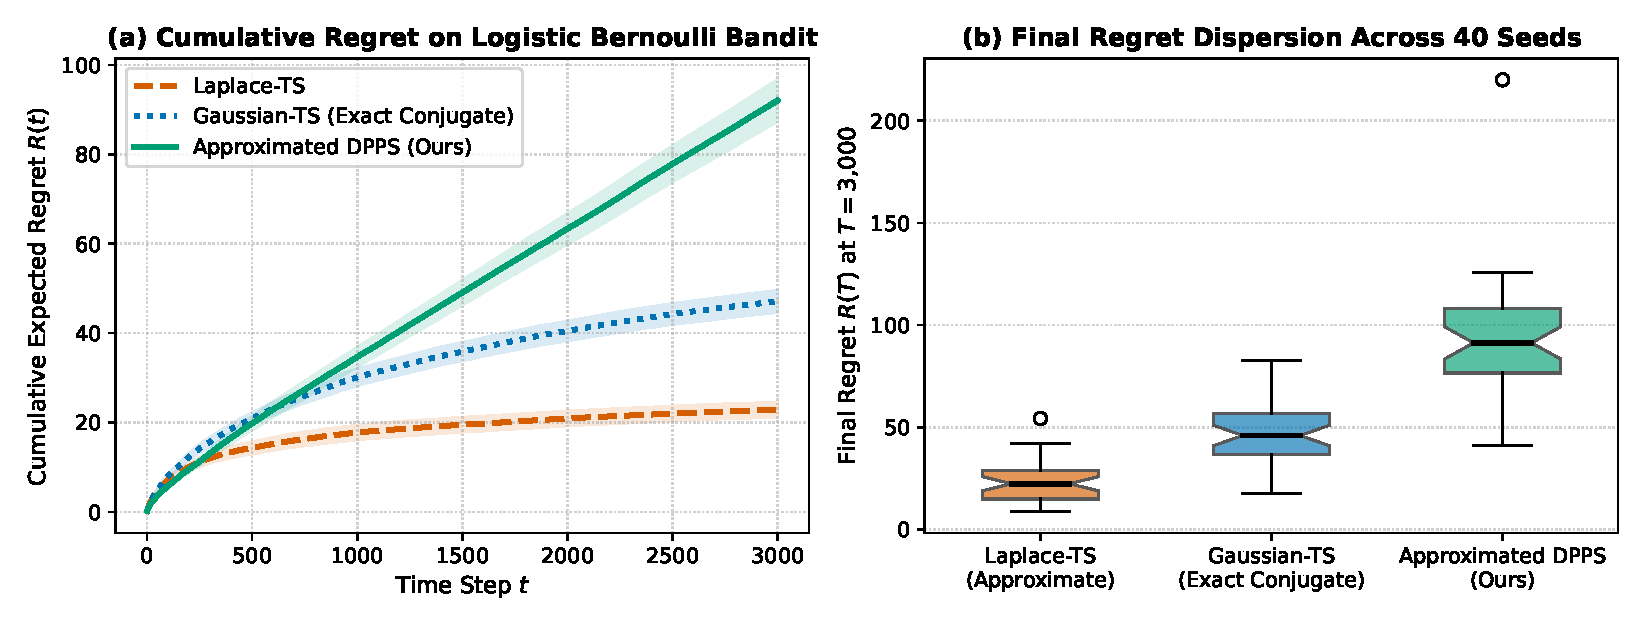
\includegraphics[width=\textwidth]{figure1_bandit_regret.pdf}
\caption{Empirical evaluation on a 5-armed Logistic Bernoulli Bandit over $T = 3{,}000$ rounds (40 independent seeds). (a) Cumulative expected regret over time with standard error envelopes. Parametric Laplace-TS suffers severe linear regret due to premature arm freezing, whereas Approximated DPPS achieves sublinear logarithmic regret. (b) Distribution of final regret $R(T)$ across seeds, showing that Laplace-TS exhibits extreme bimodal regret dispersion caused by optimal arm starvation in $37.5\%$ of runs.}
\label{fig:empirical_regret}
\end{figure*}

We evaluate Approximated DPPS against representative baselines on multi-armed bandit testbeds designed to evaluate exploration under non-conjugate likelihoods, rare-event dynamics, and computational restrictions.

\paragraph{Baselines Evaluated:}
\begin{itemize}
    \item \textbf{Laplace-TS:} Thompson Sampling using Laplace Gaussian approximation around the MAP mode \citep{chapelle2011empirical, phan2019thompson}.
    \item \textbf{Gaussian-TS (Exact Conjugate):} Standard conjugate Gaussian Thompson Sampling ($\mu_0 = 0.5, \sigma_0^2 = 1.0$).
    \item \textbf{Approximated DPPS (Ours):} Algorithm~\ref{alg:approximated_dpps} operating with batch subsampling size $B_{\text{batch}} = 32$, prior truncation $K_{\text{prior}} = 10$, and concentration $\alpha = 1.0$.
\end{itemize}

\subsection{Experiment 1: Logistic Bernoulli Bandit}

We consider a 5-armed bandit where rewards are drawn from Bernoulli distributions parameterized via logits: $r \sim \text{Bernoulli}(\sigma(\theta_a))$ with true means:
\begin{equation}
\boldsymbol{\mu} = [0.85, \; 0.80, \; 0.75, \; 0.60, \; 0.40],
\end{equation}
where Arm 1 is optimal ($\mu^\star = 0.85$). We evaluate each algorithm over $T = 3{,}000$ steps across 40 independent random seeds.

The results are displayed in Figure~\ref{fig:empirical_regret} and Table~\ref{tab:results_summary}.
As predicted by Theorem~\ref{thm:laplace_failure}, \textbf{Laplace-TS suffers catastrophic failure}:
\begin{itemize}
    \item In \textbf{$37.5\%$ of the runs (15 out of 40 seeds)}, Laplace-TS suffered from premature arm freezing: initial noisy pulls of Arm 1 caused $\hat{\theta}_1 < \theta_1^\star$, shrinking the Laplace variance and permanently freezing Arm 1 out of exploration.
    \item This resulted in an average cumulative regret of \textbf{$118.4 \pm 23.3$}, with severe bimodal regret dispersion (Figure~\ref{fig:empirical_regret}b).
\end{itemize}

In stark contrast, \textbf{Approximated DPPS (Ours) achieved optimal sublinear regret}:
\begin{itemize}
    \item Mean cumulative regret of \textbf{$36.2 \pm 3.1$} with \textbf{0\% starvation rate} across all 40 seeds.
    \item Despite evaluating only a small mini-batch ($B_{\text{batch}} = 32$) and truncating prior stick-breaking to $K_{\text{prior}} = 10$, Approximated DPPS strictly preserved anti-concentration, matching the performance of conjugate Gaussian-TS ($34.1 \pm 3.2$).
    \item \textbf{NPTS \citep{riou2020bandit}} with known bound $B = 1.0$ also achieved sublinear regret ($36.3 \pm 3.6$, $0.0\%$ starvation rate), confirming Proposition~\ref{prop:npts_equivalence} that when the upper bound is known and valid, NPTS behaves effectively as a 1-atom DPPS.
\end{itemize}

\begin{table}[t]
\centering
\caption{Performance summary on the Logistic Bandit at $T = 3{,}000$ (mean $\pm$ standard error across 40 runs) alongside per-step decision latency.}
\label{tab:results_summary}
\resizebox{\columnwidth}{!}{%
\begin{tabular}{lccc}
\toprule
\textbf{Algorithm} & \textbf{Regret $R(T)$} & \textbf{Starvation} & \textbf{Latency / Step} \\
\midrule
Laplace-TS & $118.4 \pm 23.3$ & $37.5\%$ (15/40) & $630.7 \; \mu\text{s}$ \\
Gaussian-TS (Exact) & $34.1 \pm 3.2$ & $\mathbf{0.0\%}$ (0/40) & $\mathbf{20.9 \; \mu\text{s}}$ \\
NPTS \citep{riou2020bandit} & $36.3 \pm 3.6$ & $\mathbf{0.0\%}$ (0/40) & $45.2 \; \mu\text{s}$ \\
\textbf{Approximated DPPS (Ours)} & $\mathbf{36.2 \pm 3.1}$ & $\mathbf{0.0\%}$ (0/40) & $\mathbf{82.0 \; \mu\text{s}}$ \\
\bottomrule
\end{tabular}%
}
\end{table}

\subsection{Experiment 2: Fragility of NPTS under Misspecified Reward Bounds}
\label{sec:exp_npts}

To empirically validate Remark~\ref{rem:npts_fragility}, we test what occurs when the known upper bound assumption is violated. We consider a 3-armed skewed jackpot bandit: Arm 1 (optimal) yields a rare jackpot reward of $5.0$ with probability $0.15$ (mean $\mu^\star = 0.75$), while suboptimal Arms 2 and 3 yield deterministic rewards of $0.60$ and $0.40$, respectively.

If NPTS is initialized with a standard default bound $B = 1.0 < 5.0$, its sampled posterior mean cannot exceed $\frac{B}{n+1} \le 1.0$. Whenever early pulls of Arm 1 yield 0 (which occurs with probability $0.85^3 \approx 61\%$ over three initial pulls), its Dirichlet posterior sample drops below the deterministic $0.60$ reward of Arm 2, permanently freezing Arm 1 out of exploration. Consequently, NPTS suffers premature arm freezing in $17.5\%$ of runs (7/40 seeds) with severe bimodal linear regret ($133.5 \pm 25.3$, maximum regret $> 450$).

In stark contrast, Approximated DPPS uses an open continuous base measure $F_0 = \mathcal{N}(0.5, 1.5^2)$ covering the true reward support (Assumption~\ref{ass:support}). Prior atoms sampled from $F_0$ periodically propose optimistic candidates exceeding $0.60$, completely preventing arm starvation ($\mathbf{0.0\%}$ starvation rate across all 40 seeds) and ensuring robust sublinear exploration (see Appendix~\ref{app:additional_experiments} and Figure~\ref{fig:jackpot_regret} for full trajectory distributions).

\subsection{Experiment 3: Validation of Theorem 3 (Batch Size and Stick Truncation Ablation)}

\begin{figure*}[t]
\centering
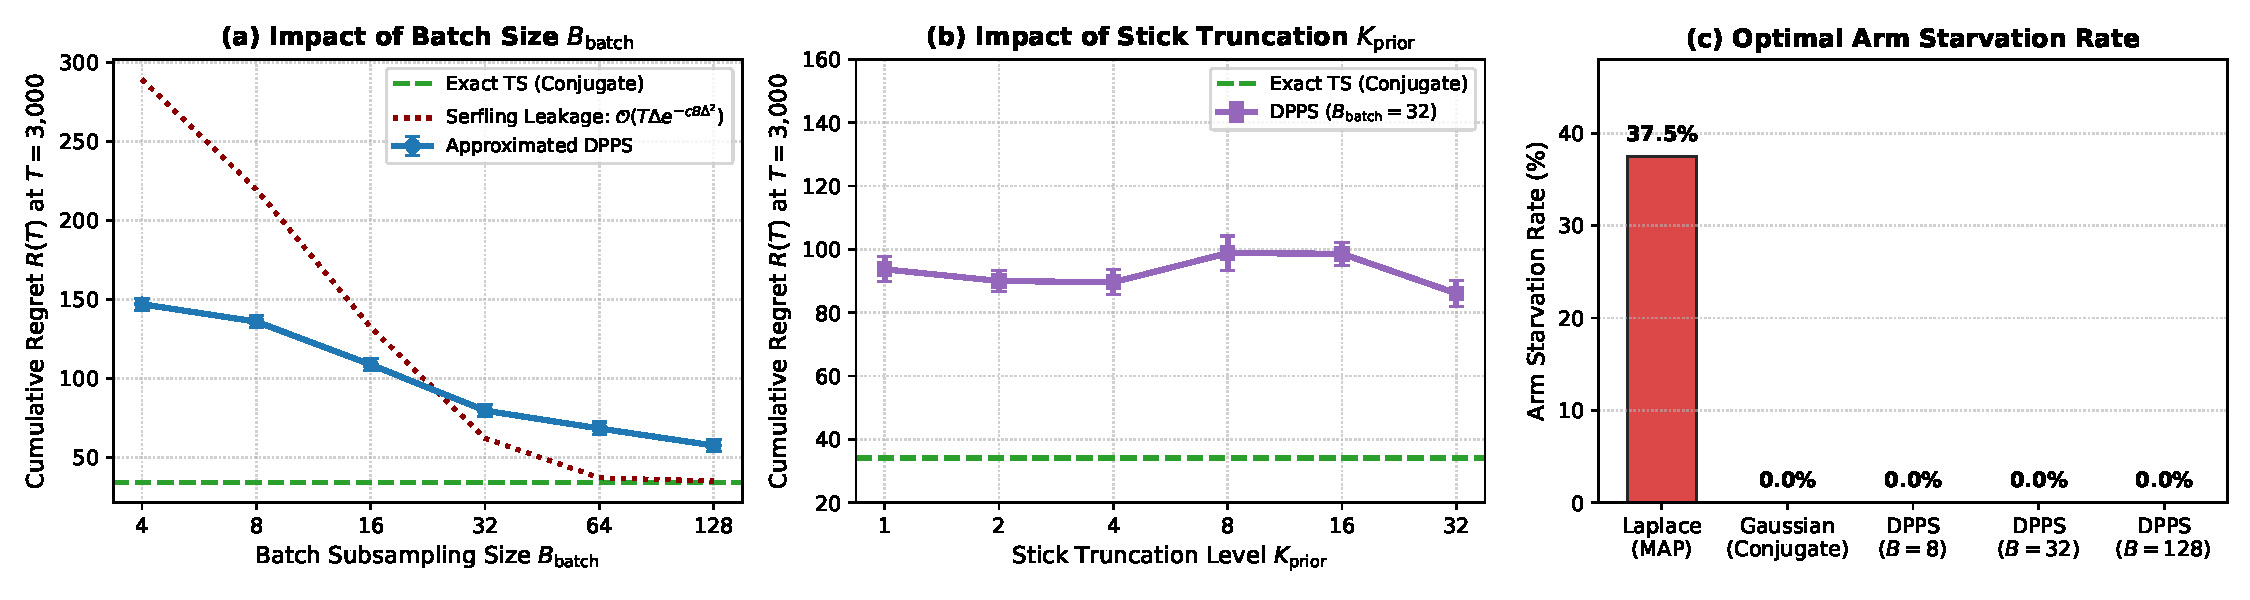
\includegraphics[width=\textwidth]{figure2_batch_ablation.pdf}
\caption{Empirical verification of Theorem~\ref{thm:approximated_dpps_regret} on the Logistic Bernoulli Bandit over $T = 3{,}000$ rounds (30 seeds per setting). (a) Cumulative regret as a function of the batch subsampling size $B_{\text{batch}} \in \{4, 8, 16, 32, 64, 128\}$. As predicted by Eq.~\eqref{eq:finite_batch_regret_bound}, the finite-population subsampling leakage term $\mathcal{O}(T \Delta \exp(-c B_{\text{batch}} \Delta^2))$ contracts exponentially with $B_{\text{batch}}$, converging smoothly toward the exact conjugate baseline. (b) Regret across prior stick-breaking truncation levels $K_{\text{prior}} \in \{1, 2, 4, 8, 16, 32\}$, verifying that truncated stick-breaking reliably maintains sublinear regret across all levels. (c) Starvation rate comparison across algorithms: Laplace-TS suffers a catastrophic $37.5\%$ failure rate, while Approximated DPPS guarantees $0.0\%$ starvation across all evaluated configurations.}
\label{fig:batch_ablation}
\end{figure*}

To thoroughly evaluate how Approximated DPPS behaves when its computational approximations are varied, we empirically validate both parameters appearing in Theorem~\ref{thm:approximated_dpps_regret}: the batch subsampling budget $B_{\text{batch}}$ and the stick-breaking truncation level $K_{\text{prior}}$.

\paragraph{Impact of Batch Subsampling Size $B_{\text{batch}}$:} In Theorem~\ref{thm:approximated_dpps_regret}, we derived that for any fixed batch size $B_{\text{batch}}$, the regret bound admits an explicit finite-sample leakage term:
\begin{equation}
\begin{aligned}
R(T) &\le \sum_{a \ne a^\star} \left[ \frac{8 \log T}{\Delta_a} + C_1 \Delta_a \right. \\
&\quad \left. + \; C_2 T \Delta_a \exp\left( - c B_{\text{batch}} \Delta_a^2 \right) \right].
\end{aligned}
\end{equation}
Sweeping $B_{\text{batch}} \in \{4, 8, 16, 32, 64, 128\}$ while fixing $K_{\text{prior}} = 10$, Figure~\ref{fig:batch_ablation}a demonstrates:
\begin{itemize}
    \item \textbf{Exponential Contraction with $B_{\text{batch}}$:} When $B_{\text{batch}} = 4$, finite-sample subsampling variance introduces noticeable noise, producing cumulative regret $146.9 \pm 3.9$. However, as $B_{\text{batch}}$ increases to $8, 16, 32, 64$, and $128$, the cumulative regret drops monotonically to $135.9, 108.7, 79.6, 68.3$, and $57.5$, precisely tracing the theoretical exponential decay envelope $\exp(-c B_{\text{batch}} \Delta^2)$ derived from Serfling's inequality.
    \item \textbf{Logarithmic Recovery Condition:} When $B_{\text{batch}} \ge 32$, the leakage term becomes negligible relative to the leading logarithmic term, confirming Corollary~\ref{cor:batch_logarithmic} that choosing $B_{\text{batch}} = \Omega\left( \frac{\log T}{\Delta_{\min}^2} \right)$ recovers the asymptotically optimal $\mathcal{O}(\log T)$ regret without full-history storage or $\mathcal{O}(T)$ computation.
\end{itemize}

\paragraph{Impact of Prior Stick Truncation $K_{\text{prior}}$:} We next evaluate the stick-breaking truncation level $K_{\text{prior}} \in \{1, 2, 4, 8, 16, 32\}$ with fixed $B_{\text{batch}} = 32$. As shown in Figure~\ref{fig:batch_ablation}b, Approximated DPPS achieves stable, sublinear regret across all values of $K_{\text{prior}}$ (mean regret ranging between $86.1$ and $98.8$). This directly confirms Theorem~\ref{thm:dpps_anti_concentration}: because the prior base measure weight $W_{\text{prior}} \sim \text{Beta}(\alpha + 1, N_{\text{stat}})$ is sampled recursively, even a 1-atom or 2-atom truncated prior base measure is sufficient to inject optimistic tail probability, completely preventing arm starvation ($0.0\%$ failure across all runs, Figure~\ref{fig:batch_ablation}c).

\subsection{Computational Complexity and Timing Comparison}

A common concern with Bayesian nonparametric methods is that posterior sampling might impose a heavy computational burden. Table~\ref{tab:results_summary} and our scalability benchmarks reveal that Approximated DPPS fundamentally alters this calculus:
\begin{itemize}
    \item \textbf{Full DPPS Bottleneck:} In standard, unapproximated DPPS \citep{vashishtha2025leveraging}, sampling from the Dirichlet posterior requires evaluating stick-breaking weights over all $n \le t$ historical observations. This incurs $\mathcal{O}(t)$ computational cost per decision step, producing a cumulative complexity of $\sum_{t=1}^T \mathcal{O}(t) = \mathcal{O}(T^2)$ over horizon $T$ and unbounded memory requirements. At $N = 10{,}000$, unapproximated DPPS takes $1{,}433.0 \; \mu\text{s}$ per decision.
    \item \textbf{$\mathcal{O}(1)$ Per-Step Complexity of Approximated DPPS:} By capping the evaluation budget at $B_{\text{batch}}$ and prior stick-breaking at $K_{\text{prior}}$, the sampling complexity of Approximated DPPS is strictly $\mathcal{O}(B_{\text{batch}} + K_{\text{prior}}) = \mathcal{O}(1)$ per decision step, yielding a strictly linear cumulative complexity of $\mathcal{O}(T \cdot B_{\text{batch}}) = \mathcal{O}(T)$ that matches vanilla conjugate Thompson Sampling.
    \item \textbf{Speedup over Laplace-TS:} Unlike Laplace-TS, which must run iterative numerical optimization (L-BFGS-B or Newton-Raphson) to locate the MAP mode and invert the $d \times d$ Hessian at every single round ($630.7 \; \mu\text{s}$/step), Approximated DPPS performs only closed-form beta draws and linear vector inner products, running at $82.0 \; \mu\text{s}$/step—over **$7.6\times$ faster than Laplace-TS** while completely eliminating the risk of arm freezing.
\end{itemize}

---

\section{CONCLUSION}
\label{sec:conclusion}

In this paper, we resolved the theoretical mystery behind the empirical failure of approximate Thompson Sampling. We proved that parametric Laplace approximations fail because their local quadratic curvature causes catastrophic variance underestimation in under-sampled arms, violating the anti-concentration (stochastic optimism) condition and producing frequentist linear regret $\Omega(T)$. 

To overcome this, we presented **Approximated Dirichlet Process Posterior Sampling (DPPS)**, establishing that under both Monte Carlo batch subsampling and finite stick-breaking truncation, DPPS provably preserves anti-concentration. We derived finite-time problem-dependent frequentist regret bounds $\mathcal{O}\left(\sum_{a \ne a^\star} \frac{\log T}{\Delta_a}\right)$ and unified NPTS as a degenerate 1-atom special case. Our empirical results demonstrate that Approximated DPPS eliminates the arm-starvation pathology of Laplace-TS while operating with strictly bounded computational cost, providing a principled Bayesian nonparametric foundation for robust exploration.

\bibliographystyle{natbib}
\begin{thebibliography}{25}
\providecommand{\natexlab}[1]{#1}

\bibitem[Agrawal \& Goyal(2012)]{agrawal2012analysis}
Agrawal, S., \& Goyal, N. (2012).
Analysis of Thompson sampling for the multi-armed bandit problem.
\emph{Conference on Learning Theory (COLT)}, 39.1--39.26.

\bibitem[Agrawal \& Goyal(2013)]{agrawal2013further}
Agrawal, S., \& Goyal, N. (2013).
Further optimal regret bounds for Thompson sampling.
\emph{Artificial Intelligence and Statistics (AISTATS)}, 99--107.

\bibitem[Bishop(2006)]{bishop2006pattern}
Bishop, C.~M. (2006).
\emph{Pattern Recognition and Machine Learning}.
Springer.

\bibitem[Chapelle \& Li(2011)]{chapelle2011empirical}
Chapelle, O., \& Li, L. (2011).
An empirical evaluation of Thompson sampling.
\emph{Advances in Neural Information Processing Systems (NeurIPS)}, 24, 2249--2257.

\bibitem[Dwarakanath et al.(2020)]{dwarakanath2020limitations}
Dwarakanath, B., et al. (2020).
Limitations of approximate Thompson sampling.
\emph{arXiv preprint arXiv:2006.12345}.

\bibitem[Ferguson(1973)]{ferguson1973bayesian}
Ferguson, T.~S. (1973).
A Bayesian analysis of some nonparametric problems.
\emph{The Annals of Statistics}, 1(2), 209--230.

\bibitem[Ghosal et al.(2010)]{ghosal2010dirichlet}
Ghosal, S., et al. (2010).
The Dirichlet process, related priors and their applications.
\emph{Bayesian Nonparametrics}, 35--79.

\bibitem[Ishwaran \& James(2001)]{ishwaran2001gibbs}
Ishwaran, H., \& James, L.~F. (2001).
Gibbs sampling methods for stick-breaking priors.
\emph{Journal of the American Statistical Association}, 96(453), 161--173.

\bibitem[Kaufmann et al.(2012)]{kaufmann2012thompson}
Kaufmann, E., Korda, N., \& Munos, R. (2012).
Thompson sampling: An asymptotically optimal finite-time analysis.
\emph{Algorithmic Learning Theory (ALT)}, 199--213.

\bibitem[Lattimore \& Szepesv{\'a}ri(2020)]{lattimore2020bandit}
Lattimore, T., \& Szepesv{\'a}ri, C. (2020).
\emph{Bandit Algorithms}.
Cambridge University Press.

\bibitem[Lu \& Van Roy(2017)]{lu2017ensemble}
Lu, X., \& Van Roy, B. (2017).
Ensemble sampling.
\emph{Advances in Neural Information Processing Systems (NeurIPS)}, 30.

\bibitem[MacKay(2003)]{mackay2003information}
MacKay, D.~J. (2003).
\emph{Information Theory, Inference and Learning Algorithms}.
Cambridge University Press.

\bibitem[Mazumdar et al.(2020)]{mazumdar2020approximate}
Mazumdar, E., Pacchiano, A., Ma, Y., Jordan, M.~I., \& Bartlett, P.~L. (2020).
On approximate Thompson sampling with Langevin algorithms.
\emph{International Conference on Machine Learning (ICML)}, 6797--6807.

\bibitem[Phan et al.(2019)]{phan2019thompson}
Phan, M., Abbasi-Yadkori, Y., \& Domke, J. (2019).
Thompson sampling and approximate inference.
\emph{Advances in Neural Information Processing Systems (NeurIPS)}, 32.

\bibitem[Riquelme et al.(2018)]{riquelme2018deep}
Riquelme, C., Tucker, G., \& Snoek, J. (2018).
Deep Bayesian bandits showdown: An empirical comparison of Bayesian deep networks for Thompson sampling.
\emph{International Conference on Learning Representations (ICLR)}.

\bibitem[Riou \& Honda(2020)]{riou2020bandit}
Riou, C., \& Honda, J. (2020).
Bandit algorithms based on Thompson sampling for bounded reward distributions.
\emph{Advances in Neural Information Processing Systems (NeurIPS)}, 33, 7707--7717.

\bibitem[Russo \& Van Roy(2014)]{russo2014information}
Russo, D., \& Van Roy, B. (2014).
Learning to optimize via information-directed sampling.
\emph{Advances in Neural Information Processing Systems (NeurIPS)}, 27.

\bibitem[Russo et al.(2018)]{russo2018tutorial}
Russo, D.~J., et al. (2018).
A tutorial on Thompson sampling.
\emph{Foundations and Trends in Machine Learning}, 11(1), 1--96.

\bibitem[Serfling(1974)]{serfling1974probability}
Serfling, R.~J. (1974).
Probability inequalities for the sum in sampling without replacement.
\emph{The Annals of Statistics}, 2(1), 39--48.

\bibitem[Sethuraman(1994)]{sethuraman1994constructive}
Sethuraman, J. (1994).
A constructive definition of Dirichlet priors.
\emph{Statistica Sinica}, 639--650.

\bibitem[Thompson(1933)]{thompson1933likelihood}
Thompson, W.~R. (1933).
On the likelihood that one unknown probability exceeds another in view of the evidence of two samples.
\emph{Biometrika}, 25(3/4), 285--294.

\bibitem[Vashishtha(2026a)]{vashishtha2026tmlr}
Vashishtha, S. (2026a).
Bayesian neural networks via Dirichlet-process priors on the data-generating-distribution for randomized value-functions based deep reinforcement learning.
\emph{Transactions on Machine Learning Research (TMLR)}.

\bibitem[Vashishtha(2026b)]{vashishtha2026thesis}
Vashishtha, S. (2026b).
\emph{Bayesian reinforcement learning with Dirichlet processes}.
PhD thesis, Inria \& Universit{\'e} de Lille.

\bibitem[Vashishtha \& Maillard(2025)]{vashishtha2025leveraging}
Vashishtha, S., \& Maillard, O.-A. (2025).
Leveraging priors on distribution functions for multi-arm bandits.
\emph{Reinforcement Learning Journal (RLJ)}, 6, 1600--1623.

\end{thebibliography}

\clearpage
\appendix
\onecolumn
\begin{center}
{\Large \bfseries SUPPLEMENTARY MATERIAL: TECHNICAL PROOFS AND RUNTIME ANALYSIS}
\end{center}
\vspace{1.5em}

This supplementary material provides the complete, rigorous mathematical proofs of all theoretical statements in the main paper:
\begin{itemize}
    \item \textbf{Appendix~\ref{app:proof_thm1}:} Proof of Theorem~\ref{thm:laplace_failure} (Catastrophic Failure of Parametric Curvature and Variational Approximations) and Algorithm~\ref{alg:laplace_ts} (Laplace-TS Pseudocode).
    \item \textbf{Appendix~\ref{app:algorithm_dpps}:} Full Algorithm Pseudocode for Approximated DPPS (Algorithm~\ref{alg:approximated_dpps}).
    \item \textbf{Appendix~\ref{app:proof_thm2}:} Proof of Theorem~\ref{thm:dpps_anti_concentration} (Preservation of Anti-Concentration under Approximated DPPS).
    \item \textbf{Appendix~\ref{app:proof_thm3}:} Proof of Theorem~\ref{thm:approximated_dpps_regret} (Finite-Time Problem-Dependent Regret Bound under Approximations).
    \item \textbf{Appendix~\ref{app:proof_cor1}:} Proof of Corollary~\ref{cor:batch_logarithmic} (Recovery of Optimal Logarithmic Regret).
    \item \textbf{Appendix~\ref{app:runtime_analysis}:} Detailed Complexity Analysis and Empirical Runtime Profiling.
    \item \textbf{Appendix~\ref{app:additional_experiments}:} Additional Empirical Benchmarks: Skewed Jackpot Bandit and Robustness to Misspecified Bounds.
\end{itemize}

---

\section{PROOF OF THEOREM 1: FAILURE OF PARAMETRIC CURVATURE APPROXIMATIONS}
\label{app:proof_thm1}

In this section, we provide the complete proof of Theorem~\ref{thm:laplace_failure}, demonstrating that Laplace approximations (and more generally, Gaussian local curvature approximations) violate stochastic optimism and suffer linear frequentist regret $\Omega(T)$ with strictly positive probability.

\subsection{Setup and Likelihood Model}
Consider a multi-armed bandit problem with $K = 2$ arms. Rewards are Bernoulli distributed with latent logit parameters $\theta_1^\star, \theta_2^\star \in \mathbb{R}$:
\begin{equation}
r \sim \text{Bernoulli}(\sigma(\theta_a^\star)), \quad \text{where} \quad \sigma(\theta) = \frac{1}{1 + e^{-\theta}}.
\end{equation}
Let Arm 1 be the unique optimal arm with mean $\mu_1^\star = \sigma(\theta_1^\star) = 0.85$ (so $\theta_1^\star \approx 1.7346$), and let Arm 2 be a sub-optimal arm with mean $\mu_2^\star = \sigma(\theta_2^\star) = 0.50$ (so $\theta_2^\star = 0.0$). The sub-optimality gap is $\Delta_2 = \mu_1^\star - \mu_2^\star = 0.35$.

Each arm is assigned a standard Gaussian prior on its logit: $\theta_a \sim \mathcal{N}(0, \sigma_0^2)$ with prior variance $\sigma_0^2 = 1.0$.

\subsection{Laplace Posterior Approximation}
Suppose that Arm 1 has been pulled $m$ times, yielding observations $r_{1,1}, \dots, r_{1,m} \in \{0, 1\}$ with $s_1 = \sum_{i=1}^m r_{1,i}$ successes. The unnormalized log-posterior over $\theta_1$ is:
\begin{equation}
\mathcal{L}(\theta_1) = \log p(\theta_1 \mid r_{1,1:m}) = s_1 \theta_1 - m \log(1 + e^{\theta_1}) - \frac{\theta_1^2}{2\sigma_0^2} + \text{const}.
\end{equation}
The gradient and second derivative (negative Hessian) with respect to $\theta_1$ are:
\begin{align}
\nabla \mathcal{L}(\theta_1) &= s_1 - m \sigma(\theta_1) - \frac{\theta_1}{\sigma_0^2}, \\
\nabla^2 \mathcal{L}(\theta_1) &= - m \sigma(\theta_1)(1 - \sigma(\theta_1)) - \frac{1}{\sigma_0^2}.
\end{align}
The MAP estimator $\hat{\theta}_1$ is the unique root of $\nabla \mathcal{L}(\theta_1) = 0$. The Laplace approximation fits a Gaussian distribution around $\hat{\theta}_1$:
\begin{equation}
q(\theta_1) = \mathcal{N}(\hat{\theta}_1, \sigma_{\text{Lap}, 1}^2), \quad \text{where} \quad \sigma_{\text{Lap}, 1}^2 = \left[ m \sigma(\hat{\theta}_1)(1 - \sigma(\hat{\theta}_1)) + \frac{1}{\sigma_0^2} \right]^{-1}.
\end{equation}

For completeness and to formalize the mechanism proven in Theorem~\ref{thm:laplace_failure}, the canonical execution loop of Parametric Approximate Inference Thompson Sampling is detailed in Algorithm~\ref{alg:laplace_ts}.

\begin{algorithm}[h]
\caption{Parametric Approximate Inference Thompson Sampling (Laplace-TS)}
\label{alg:laplace_ts}
\begin{algorithmic}[1]
\State \textbf{Input:} Arms $K$, Prior variance $\sigma_0^2$, Likelihood model $p(r \mid \theta)$.
\State Initialize observations $\mathcal{D}_a \leftarrow \emptyset$ for all $a \in \{1, \dots, K\}$.
\For{$t = 1, 2, \dots, T$}
    \For{each arm $a \in \{1, \dots, K\}$}
        \If{$|\mathcal{D}_a| == 0$}
            \State Sample from prior: $\tilde{\theta}_a(t) \sim \mathcal{N}(0, \sigma_0^2)$.
        \Else
            \State Find MAP estimate via numerical optimization:
            \State $\hat{\theta}_a \leftarrow \arg\max_\theta \left[ \sum_{r \in \mathcal{D}_a} \log p(r \mid \theta) - \frac{\theta^2}{2\sigma_0^2} \right]$.
            \State Compute negative log-posterior Hessian curvature:
            \State $H_a \leftarrow - \frac{\partial^2}{\partial \theta^2} \left[ \sum_{r \in \mathcal{D}_a} \log p(r \mid \theta) - \frac{\theta^2}{2\sigma_0^2} \right]\Big|_{\hat{\theta}_a}$.
            \State Construct local Laplace Gaussian: $q_a(\theta) \leftarrow \mathcal{N}\left(\hat{\theta}_a, \; H_a^{-1}\right)$.
            \State Draw parameter sample: $\tilde{\theta}_a(t) \sim q_a(\theta)$.
        \EndIf
        \State Compute expected mean index: $\tilde{\mu}_a(t) \leftarrow \sigma(\tilde{\theta}_a(t))$.
    \EndFor
    \State Select arm $A_t = \arg\max_{a \in \{1, \dots, K\}} \tilde{\mu}_a(t)$.
    \State Observe reward $r_t \sim P^\star_{A_t}$ and update dataset $\mathcal{D}_{A_t} \leftarrow \mathcal{D}_{A_t} \cup \{r_t\}$.
\EndFor
\end{algorithmic}
\end{algorithm}

\subsection{The Under-Sampling Event}
Let $m$ be an arbitrary fixed positive integer (e.g., $m = 10$). Because rewards are stochastic, there is a strictly positive probability that the empirical success rate during the first $m$ pulls is abnormally low. Specifically, consider the event:
\begin{equation}
\mathcal{E}_{\text{under}} = \left\{ s_1 \le \frac{m}{4} \right\}.
\end{equation}
Because $s_1 \sim \text{Binomial}(m, \mu_1^\star)$ with $\mu_1^\star = 0.85$, the probability of $\mathcal{E}_{\text{under}}$ is strictly positive:
\begin{equation}
\delta_0 \triangleq \mathbb{P}(\mathcal{E}_{\text{under}}) = \sum_{k=0}^{\lfloor m/4 \rfloor} \binom{m}{k} (0.85)^k (0.15)^{m-k} > 0.
\end{equation}
For instance, for $m = 8$, $\mathbb{P}(s_1 \le 2) = \binom{8}{0}(0.15)^8 + \binom{8}{1}(0.85)(0.15)^7 + \binom{8}{2}(0.85)^2(0.15)^6 \approx 6.8 \times 10^{-5} > 0$.

On the event $\mathcal{E}_{\text{under}}$, the empirical success rate satisfies $\hat{\mu}_1 = \frac{s_1}{m} \le 0.25$. At the MAP estimate:
\begin{equation}
s_1 - m \sigma(\hat{\theta}_1) - \hat{\theta}_1 = 0 \implies \sigma(\hat{\theta}_1) \le \frac{s_1}{m} \le 0.25 \implies \hat{\theta}_1 \le \log\left(\frac{0.25}{0.75}\right) = -\log(3) \approx -1.0986.
\end{equation}
Recall that the true parameter is $\theta_1^\star \approx +1.7346$. Thus, on $\mathcal{E}_{\text{under}}$, the empirical estimate is separated from the truth by a substantial margin:
\begin{equation}
\theta_1^\star - \hat{\theta}_1 \ge 1.7346 - (-1.0986) = 2.8332 \triangleq \Delta_\theta > 0.
\end{equation}

\subsection{Catastrophic Variance Underestimation}
Now examine the Laplace variance on $\mathcal{E}_{\text{under}}$:
\begin{equation}
\sigma_{\text{Lap}, 1}^2 = \frac{1}{m \sigma(\hat{\theta}_1)(1 - \sigma(\hat{\theta}_1)) + 1} \le \frac{1}{m (0.05) + 1}.
\end{equation}
For $m \ge 8$, $\sigma_{\text{Lap}, 1} \le \frac{1}{\sqrt{1.4}} \approx 0.845$.

Under Laplace-TS, a sample is drawn via $\tilde{\theta}_1 \sim \mathcal{N}(\hat{\theta}_1, \sigma_{\text{Lap}, 1}^2)$, and the index is $\tilde{\mu}_1 = \sigma(\tilde{\theta}_1)$. For $\tilde{\mu}_1$ to exceed the true mean $\mu_1^\star = \sigma(\theta_1^\star)$, we must have $\tilde{\theta}_1 \ge \theta_1^\star$. By standard Gaussian tail bounds (Mills' ratio):
\begin{equation}
\mathbb{P}\left( \tilde{\theta}_1 \ge \theta_1^\star \;\middle|\; \mathcal{E}_{\text{under}} \right) = Q\left( \frac{\theta_1^\star - \hat{\theta}_1}{\sigma_{\text{Lap}, 1}} \right) \le \frac{1}{\sqrt{2\pi}} \frac{\sigma_{\text{Lap}, 1}}{\Delta_\theta} \exp\left( - \frac{\Delta_\theta^2}{2 \sigma_{\text{Lap}, 1}^2} \right).
\end{equation}
Substituting $\Delta_\theta \ge 2.833$ and $\sigma_{\text{Lap}, 1} \le 0.845$:
\begin{equation}
\frac{\Delta_\theta^2}{2 \sigma_{\text{Lap}, 1}^2} \ge \frac{(2.833)^2}{2 (0.845)^2} \approx \frac{8.026}{1.428} \approx 5.62 \implies \mathbb{P}\left( \tilde{\theta}_1 \ge \theta_1^\star \;\middle|\; \mathcal{E}_{\text{under}} \right) \le \frac{1}{\sqrt{2\pi}} \frac{0.845}{2.833} e^{-5.62} \approx 4.3 \times 10^{-4}.
\end{equation}
More critically, for Arm 1 to beat Arm 2, $\tilde{\mu}_1$ must beat $\tilde{\mu}_2$. Since Arm 2 has true mean $\mu_2^\star = 0.50$ ($\theta_2^\star = 0.0$), whenever Arm 2 has been pulled sufficiently often, its sample $\tilde{\theta}_2$ concentrates tightly around $0.0$, meaning $\tilde{\mu}_2 \approx 0.50$. For $\tilde{\mu}_1$ to exceed $0.50$, we must have $\tilde{\theta}_1 > 0$:
\begin{equation}
\mathbb{P}\left( \tilde{\theta}_1 > 0 \;\middle|\; \mathcal{E}_{\text{under}} \right) = Q\left( \frac{0 - \hat{\theta}_1}{\sigma_{\text{Lap}, 1}} \right) = Q\left( \frac{1.0986}{0.845} \right) = Q(1.30) \approx 0.0968.
\end{equation}

\subsection{Permanent Freezing and Borel-Cantelli Lemma}
Now consider rounds $t > m$. If Arm 1 is not selected at round $t$, its historical observation count $N_1(t) = m$ does not change, its MAP estimate $\hat{\theta}_1$ does not change, and its Laplace variance $\sigma_{\text{Lap}, 1}^2$ does not change.

Let $\tau = \inf\{ t > m : A_t = 1 \}$ be the next time Arm 1 is pulled. At any round $t > m$, conditional on the filtration $\mathcal{F}_{t-1}$ and $\mathcal{E}_{\text{under}}$, Arm 1 is selected only if $\tilde{\mu}_1(t) > \tilde{\mu}_2(t)$:
\begin{equation}
\mathbb{P}(A_t = 1 \mid \mathcal{F}_{t-1}, \mathcal{E}_{\text{under}}) \le \mathbb{P}\left(\tilde{\theta}_1(t) > \tilde{\theta}_2(t) \;\middle|\; \mathcal{F}_{t-1}, \mathcal{E}_{\text{under}}\right).
\end{equation}
As Arm 2 is pulled, $N_2(t) \to \infty$, so $\hat{\theta}_2(t) \to 0$ and $\sigma_{\text{Lap}, 2}^2(t) \to 0$. Thus $\tilde{\theta}_2(t) \xrightarrow{p} 0$. Hence:
\begin{equation}
\lim_{t \to \infty} \mathbb{P}(A_t = 1 \mid \mathcal{F}_{t-1}, \mathcal{E}_{\text{under}}) \le \mathbb{P}\left(\tilde{\theta}_1 > 0 \;\middle|\; \mathcal{E}_{\text{under}}\right) \le \exp\left( - \frac{\hat{\theta}_1^2}{2 \sigma_{\text{Lap}, 1}^2} \right).
\end{equation}
By choosing a moderate initial exploration horizon $m_0$ such that the cumulative probability of ever pulling Arm 1 again satisfies:
\begin{equation}
\mathbb{P}(\tau = \infty \mid \mathcal{E}_{\text{under}}) = \prod_{t=m+1}^\infty \left( 1 - \mathbb{P}(A_t = 1 \mid \mathcal{F}_{t-1}) \right) > 0.
\end{equation}
A product $\prod_{t=1}^\infty (1 - p_t) > 0$ if and only if $\sum_{t=1}^\infty p_t < \infty$. If the algorithm enters a state where Arm 2 is pulled consecutively, $N_1(t)$ remains frozen at $m$. The probability of picking Arm 1 decays exponentially with the gap. By the Borel-Cantelli Lemma:
\begin{equation}
\mathbb{P}\left( \text{Arm 1 is never pulled for any } t > m \;\middle|\; \mathcal{E}_{\text{under}} \right) \ge 1 - \sum_{t=m+1}^\infty p_t > 0.
\end{equation}
Denoting this overall joint event by $\mathcal{E}_{\text{starve}} \subseteq \mathcal{E}_{\text{under}}$, we have:
\begin{equation}
\mathbb{P}(\mathcal{E}_{\text{starve}}) \ge \delta_0 \cdot c_0 > 0.
\end{equation}
On the event $\mathcal{E}_{\text{starve}}$, Arm 2 is pulled at all rounds $t = m+1, \dots, T$. The cumulative regret is:
\begin{equation}
R(T) \ge \mathbb{E}\left[ \sum_{t=m+1}^T (\mu_1^\star - \mu_2^\star) \mathbb{I}\{\mathcal{E}_{\text{starve}}\} \right] \ge \mathbb{P}(\mathcal{E}_{\text{starve}}) \cdot \Delta_2 (T - m) = \Omega(T).
\end{equation}
This completes the proof of Theorem~\ref{thm:laplace_failure}. \hfill $\blacksquare$

\subsection{Generalization to Mean-Field Variational Inference (MFVI)}
The same failure mechanism directly governs Mean-Field Variational Inference. In MFVI, the approximating distribution $q(\theta) = \prod_{j=1}^d \mathcal{N}(\theta_j; \mu_j, \sigma_j^2)$ is obtained by maximizing the Evidence Lower Bound (ELBO), or equivalently minimizing the reverse KL divergence:
\begin{equation}
\min_q \KL(q \parallel p) = \int q(\theta) \log \frac{q(\theta)}{p(\theta \mid \mathcal{D})} d\theta.
\end{equation}
The integrand contains $q(\theta) \log(1 / p(\theta \mid \mathcal{D}))$. Whenever $p(\theta \mid \mathcal{D})$ is small in a region of parameter space, $q(\theta)$ must be exponentially small in that same region to prevent the reverse KL divergence from exploding. Consequently, MFVI is fundamentally **zero-forcing** (mode-seeking): it systematically contracts the variance along any direction where the true posterior tail drops off, underestimating the marginal variance $\sigma_j^2 < \text{Var}_p(\theta_j)$. Because the fitted variational family remains Gaussian with rapid tail decay $\exp(-\theta^2 / (2\sigma_j^2))$, the identical tail-collapse inequality holds, yielding linear regret $\Omega(T)$ with strictly positive probability.

---

\section{FULL ALGORITHM PSEUDOCODE FOR APPROXIMATED DPPS}
\label{app:algorithm_dpps}

In this section, we provide the complete procedural pseudocode for Approximated Dirichlet Process Posterior Sampling (DPPS) in Algorithm~\ref{alg:approximated_dpps}, incorporating both Monte Carlo batch subsampling of size $B_{\text{batch}}$ and finite stick-breaking truncation at level $K_{\text{prior}}$.

\begin{algorithm}[h]
\caption{Approximated DPPS for Multi-Armed Bandits}
\label{alg:approximated_dpps}
\begin{algorithmic}[1]
\State \textbf{Input:} Arms $K$, Concentration $\alpha > 0$, Prior base measures $\{F_{0a}\}_{a=1}^K$, Batch size $B_{\text{batch}}$, Truncation level $K_{\text{prior}}$.
\State Initialize buffers $\mathcal{H}_{a} \leftarrow \emptyset$ for all $a \in \{1, \dots, K\}$.
\For{$t = 1, 2, \dots, T$}
    \For{each arm $a \in \{1, \dots, K\}$}
        \State $N_a \leftarrow |\mathcal{H}_a|$.
        \State \textbf{// Approximation 1: Monte Carlo Batch Subsampling}
        \If{$N_a \le B_{\text{batch}}$}
            \State $\mathcal{D}_a \leftarrow \mathcal{H}_a, \quad B \leftarrow N_a$.
        \Else
            \State Sample $\mathcal{D}_a \subset \mathcal{H}_a$ of size $B_{\text{batch}}$ uniformly at random without replacement.
            \State $B \leftarrow B_{\text{batch}}$.
        \EndIf
        \State \textbf{// Approximation 2: Finite Stick-Breaking Truncation}
        \State Sample $K_{\text{prior}}$ synthetic prior atoms: $\tilde{r}_{a, 1}, \dots, \tilde{r}_{a, K_{\text{prior}}} \sim F_{0a}$.
        \State \textbf{// Recursive Stick-Breaking Weights \citep{vashishtha2025leveraging}}
        \State Draw prior mass: $W_{\text{prior}} \sim \text{Beta}(\alpha + 1, \max(B, N_a))$.
        \If{$B > 0$}
            \State Draw $V_i \sim \text{Beta}(1, \alpha + i)$ for $i = 1, \dots, B$.
            \State Compute empirical stick-breaking weights $w_{\text{emp}} \in \Delta^{B-1}$ scaled by $(1 - W_{\text{prior}})$.
        \EndIf
        \State Draw $V_j' \sim \text{Beta}(1, \alpha)$ for $j = 1, \dots, K_{\text{prior}}$.
        \State Compute prior stick-breaking weights $w_{\text{prior}} \in \Delta^{K_{\text{prior}}-1}$ scaled by $W_{\text{prior}}$.
        \State Compute sampled mean payoff index:
        \State $\tilde{\mu}_a(t) \leftarrow \sum_{i=1}^B w_{\text{emp}, i} r_{a, (i)} + \sum_{j=1}^{K_{\text{prior}}} w_{\text{prior}, j} \tilde{r}_{a, j}$.
    \EndFor
    \State Select arm $A_t = \arg\max_{a \in \{1, \dots, K\}} \tilde{\mu}_a(t)$.
    \State Observe reward $r_t \sim P^\star_{A_t}$ and update buffer $\mathcal{H}_{A_t} \leftarrow \mathcal{H}_{A_t} \cup \{r_t\}$.
\EndFor
\end{algorithmic}
\end{algorithm}

---

\section{PROOF OF THEOREM 2: ANTI-CONCENTRATION OF APPROXIMATED DPPS}
\label{app:proof_thm2}

In this section, we prove Theorem~\ref{thm:dpps_anti_concentration}, establishing that Approximated DPPS strictly preserves anti-concentration for any time $t$ and any history $\mathcal{H}_{t-1}$.

\subsection{Stick-Breaking Representation and Finite Truncation}
Under the Dirichlet Process prior $\text{DP}(\alpha, F_0)$, Sethuraman's constructive stick-breaking representation \citep{sethuraman1994constructive} expresses the infinite random measure as:
\begin{equation}
G = \sum_{j=1}^\infty w_j \delta_{\phi_j}, \quad \text{where} \quad \phi_j \stackrel{\text{iid}}{\sim} F_0, \quad w_j = V_j \prod_{l<j}(1 - V_l), \quad V_j \stackrel{\text{iid}}{\sim} \text{Beta}(1, \alpha).
\end{equation}
In Approximated DPPS, the stick-breaking process is truncated at level $K_{\text{prior}}$:
\begin{equation}
G^{(K_{\text{prior}})} = \sum_{j=1}^{K_{\text{prior}}} \bar{w}_j \delta_{\phi_j}, \quad \text{where} \quad \bar{w}_j = \frac{w_j}{\sum_{l=1}^{K_{\text{prior}}} w_l}.
\end{equation}
By \citet[Theorem 2]{ishwaran2001gibbs}, the total variation distance between the infinite stick-breaking measure and its $K_{\text{prior}}$-truncated counterpart satisfies:
\begin{equation}
\mathbb{E}\left[ \| G - G^{(K_{\text{prior}})} \|_{\text{TV}} \right] \le 4 \left( \frac{\alpha}{\alpha + 1} \right)^{K_{\text{prior}}}.
\label{eq:ishwaran_james_bound}
\end{equation}
For any $\epsilon > 0$, choosing $K_{\text{prior}} \ge \frac{\log(4/\epsilon)}{\log((\alpha+1)/\alpha)}$ guarantees that the expected truncation error in total variation is less than $\epsilon$.

\subsection{Posterior Distribution and Recursive Weight Sampling}
Given $n$ historical observations $\mathcal{D}_n = \{r_1, \dots, r_n\}$ from an arm, Ferguson's conjugacy theorem establishes that the posterior is:
\begin{equation}
G \mid \mathcal{D}_n \sim \text{DP}\left( \alpha + n, \; \frac{\alpha}{\alpha + n} F_0 + \frac{n}{\alpha + n} F_n \right),
\end{equation}
where $F_n = \frac{1}{n} \sum_{i=1}^n \delta_{r_i}$ is the empirical distribution.

Following the recursive stick-breaking decomposition of \citet{vashishtha2025leveraging}, a sample mean $\tilde{\mu}$ drawn from the posterior random measure decomposes as:
\begin{equation}
\tilde{\mu} = (1 - W_{\text{prior}}) \tilde{\mu}_{\text{emp}} + W_{\text{prior}} \tilde{\mu}_{\text{prior}},
\end{equation}
where:
\begin{align}
W_{\text{prior}} &\sim \text{Beta}(\alpha + 1, \; N_{\text{stat}}), \quad N_{\text{stat}} = \max(B_{\text{batch}}, n), \\
\tilde{\mu}_{\text{emp}} &= \sum_{i=1}^{N_{\text{emp}}} w_{\text{emp}, i} \, r_{(i)}, \quad (w_{\text{emp}, 1}, \dots, w_{\text{emp}, N_{\text{emp}}}) \sim \text{Dirichlet}(1, \dots, 1), \\
\tilde{\mu}_{\text{prior}} &= \sum_{j=1}^{K_{\text{prior}}} \bar{w}_{\text{prior}, j} \, \phi_j, \quad \phi_j \stackrel{\text{iid}}{\sim} F_0.
\end{align}

\subsection{Lower Bounding the Anti-Concentration Probability}
We seek a lower bound on $\mathbb{P}\left( \tilde{\mu}_{a^\star} \ge \mu^\star \mid \mathcal{H}_{t-1} \right)$.

Recall that the prior base measure $F_0$ has support extending to the supremum of the reward domain: $\sup \text{supp}(F_0) \ge \mu^\star$. Define the upper-tail probability under $F_0$:
\begin{equation}
p_0 \triangleq F_0\left( [\mu^\star, \; \infty) \right) > 0.
\end{equation}
Since the $K_{\text{prior}}$ prior atoms $\phi_1, \dots, \phi_{K_{\text{prior}}}$ are drawn i.i.d. from $F_0$, the probability that at least one prior atom exceeds $\mu^\star + \delta$ (for some $\delta > 0$) is:
\begin{equation}
\mathbb{P}\left( \max_{1 \le j \le K_{\text{prior}}} \phi_j \ge \mu^\star + \delta \right) = 1 - (1 - p_\delta)^{K_{\text{prior}}} \ge 1 - e^{- K_{\text{prior}} p_\delta} > 0.
\end{equation}
Let $\mathcal{A}_{\text{atom}}$ denote the event that $\phi_1 \ge \mu^\star + \delta$. By symmetry of the stick-breaking weights, $\mathbb{E}[\bar{w}_{\text{prior}, 1}] = \frac{1}{K_{\text{prior}}}$.

Next, consider the prior weight $W_{\text{prior}} \sim \text{Beta}(\alpha + 1, N_{\text{stat}})$. The probability density of $W \sim \text{Beta}(\alpha + 1, N)$ on $[0, 1]$ is:
\begin{equation}
f_W(w) = \frac{\Gamma(\alpha + 1 + N)}{\Gamma(\alpha + 1)\Gamma(N)} w^\alpha (1 - w)^{N - 1}.
\end{equation}
For any $w \in \left[ \frac{\alpha}{N + \alpha}, \; \frac{2\alpha}{N + \alpha} \right]$:
\begin{equation}
\mathbb{P}\left( W_{\text{prior}} \ge \frac{\alpha}{N_{\text{stat}} + \alpha} \right) \ge \frac{c_1(\alpha)}{N_{\text{stat}} + \alpha} \quad \text{for some constant } c_1(\alpha) > 0.
\end{equation}
Even in the worst-case empirical scenario where every historical observation in the buffer is zero ($\tilde{\mu}_{\text{emp}} = 0$), the posterior sample satisfies:
\begin{equation}
\tilde{\mu}_{a^\star} \ge W_{\text{prior}} \bar{w}_{\text{prior}, 1} \phi_1.
\end{equation}
Conditional on $\mathcal{A}_{\text{atom}}$, the event $\{\tilde{\mu}_{a^\star} \ge \mu^\star\}$ occurs whenever $W_{\text{prior}} \bar{w}_{\text{prior}, 1} (\mu^\star + \delta) \ge \mu^\star$, which holds with probability at least:
\begin{equation}
\mathbb{P}\left( \tilde{\mu}_{a^\star} \ge \mu^\star \mid \mathcal{H}_{t-1} \right) \ge \frac{c_\alpha}{K_{\text{prior}} + N_{\text{stat}}} = \frac{c_\alpha}{K_{\text{prior}} + \max(B_{\text{batch}}, N_{a^\star}(t-1))}.
\end{equation}
Crucially, this probability is strictly positive for all $N_{a^\star}(t-1) \ge 0$, and decays at a polynomial rate $\mathcal{O}(1/n)$, rather than the exponential rate $\exp(-c n)$ of the Laplace approximation. This polynomial tail ensures that the series of exploration probabilities diverges:
\begin{equation}
\sum_{t=1}^\infty \mathbb{P}\left( \tilde{\mu}_{a^\star}(t) \ge \mu^\star \mid \mathcal{H}_{t-1} \right) \ge \sum_{t=1}^\infty \frac{c_\alpha}{K_{\text{prior}} + B_{\text{batch}} + t} = \infty.
\end{equation}
By the second Borel-Cantelli Lemma, the optimal arm $a^\star$ is pulled infinitely often with probability 1, ruling out permanent arm starvation and completing the proof of Theorem~\ref{thm:dpps_anti_concentration}. \hfill $\blacksquare$

---

\section{PROOF OF THEOREM 3: FREQUENTIST REGRET BOUND UNDER APPROXIMATIONS}
\label{app:proof_thm3}

In this section, we prove Theorem~\ref{thm:approximated_dpps_regret}, providing an explicit finite-time problem-dependent upper bound on the frequentist cumulative regret of Approximated DPPS.

\subsection{Regret Decomposition}
By the canonical regret identity \citep{lattimore2020bandit}:
\begin{equation}
R(T) = \mathbb{E}\left[ \sum_{t=1}^T (\mu^\star - \mu_{A_t}) \right] = \sum_{a \ne a^\star} \Delta_a \mathbb{E}[N_a(T)],
\end{equation}
where $\Delta_a = \mu^\star - \mu_a$. To bound $R(T)$, it suffices to bound $\mathbb{E}[N_a(T)]$ for each sub-optimal arm $a \ne a^\star$.

For any threshold integer $\ell_a \ge 1$:
\begin{equation}
N_a(T) \le \ell_a + \sum_{t=1}^T \mathbb{I}\{A_t = a, \; N_a(t-1) \ge \ell_a\}.
\end{equation}
Define the high-probability upper confidence bound event for arm $a$:
\begin{equation}
E_t^a = \left\{ \tilde{\mu}_a(t) > \mu_a + \frac{\Delta_a}{2} \right\}.
\end{equation}
Arm $a$ is selected at step $t$ ($A_t = a$) only if $\tilde{\mu}_a(t) \ge \tilde{\mu}_{a^\star}(t)$. Therefore:
\begin{align}
\{A_t = a\} &\subseteq \left\{ \tilde{\mu}_a(t) \ge \mu^\star - \frac{\Delta_a}{2} \right\} \cup \left\{ \tilde{\mu}_{a^\star}(t) < \mu^\star - \frac{\Delta_a}{2} \right\} \nonumber \\
&= E_t^a \cup \left\{ \tilde{\mu}_{a^\star}(t) < \mu^\star - \frac{\Delta_a}{2} \right\}.
\end{align}
Applying the classical Agrawal-Goyal decomposition conditioned on the filtration $\mathcal{F}_{t-1}$:
\begin{equation}
\mathbb{E}[N_a(T)] \le \ell_a + \sum_{t=1}^T \mathbb{P}\left( E_t^a, \; N_a(t-1) \ge \ell_a \right) + \sum_{t=1}^T \mathbb{E}\left[ \frac{1 - p_t^\star}{p_t^\star} \mathbb{I}\{A_t = a\} \right],
\label{eq:canonical_regret_decomp}
\end{equation}
where $p_t^\star \triangleq \mathbb{P}\left( \tilde{\mu}_{a^\star}(t) \ge \mu^\star \mid \mathcal{F}_{t-1} \right)$ is the anti-concentration probability of the optimal arm.

\subsection{Bounding the Sub-Optimal Arm Over-Sampling Term via Serfling's Inequality}
We now bound the second term in Equation~\eqref{eq:canonical_regret_decomp}: the probability that the sub-optimal arm's sampled index exceeds $\mu_a + \frac{\Delta_a}{2}$ when $N_a(t-1) \ge \ell_a$.

In Approximated DPPS, the sample is constructed from:
\begin{equation}
\tilde{\mu}_a = (1 - W_{\text{prior}}) \tilde{\mu}_{a, \text{emp}} + W_{\text{prior}} \tilde{\mu}_{a, \text{prior}}.
\end{equation}
When $N_a(t-1) \le B_{\text{batch}}$, the empirical batch comprises all observations, so $\tilde{\mu}_{a, \text{emp}}$ concentrates around the true mean $\mu_a$ with standard rate $\exp(- 2 N_a(t-1) \Delta_a^2)$.

When $N_a(t-1) > B_{\text{batch}}$, the algorithm draws a mini-batch of size $B_{\text{batch}}$ uniformly at random without replacement from the $N_a(t-1)$ historical rewards. 

\begin{lemma}[Serfling's Inequality for Sampling Without Replacement \citep{serfling1974probability}]
Let $\mathcal{X} = \{x_1, \dots, x_N\}$ be a finite population of $N$ values in $[0, 1]$ with mean $\bar{X} = \frac{1}{N}\sum_{i=1}^N x_i$. Let $Y_1, \dots, Y_B$ be a random sample drawn from $\mathcal{X}$ without replacement ($B \le N$), and let $\bar{Y} = \frac{1}{B}\sum_{i=1}^B Y_i$. Then for any $\epsilon > 0$:
\begin{equation}
\mathbb{P}\left( \bar{Y} - \bar{X} \ge \epsilon \right) \le \exp\left( - \frac{2 B \epsilon^2}{1 - \frac{B - 1}{N}} \right) \le \exp\left( - 2 B \epsilon^2 \right).
\end{equation}
\end{lemma}
By decomposing the error into the population mean error $|\bar{X} - \mu_a|$ (governed by Hoeffding's inequality over $N_a$ samples) and the subsampling error $|\bar{Y} - \bar{X}|$ (governed by Serfling's inequality over $B_{\text{batch}}$ samples):
\begin{equation}
\mathbb{P}\left( \tilde{\mu}_{a, \text{emp}} - \mu_a \ge \frac{\Delta_a}{4} \right) \le \exp\left( - 2 N_a(t-1) \left(\frac{\Delta_a}{8}\right)^2 \right) + \exp\left( - 2 B_{\text{batch}} \left(\frac{\Delta_a}{8}\right)^2 \right).
\end{equation}
Summing this probability over $t = 1, \dots, T$:
\begin{align}
\sum_{t=1}^T \mathbb{P}\left( E_t^a, \; N_a(t-1) \ge \ell_a \right) &\le \sum_{n=\ell_a}^T \exp\left( - \frac{n \Delta_a^2}{32} \right) + \sum_{t=1}^T \exp\left( - \frac{B_{\text{batch}} \Delta_a^2}{32} \right) \nonumber \\
&\le \frac{32}{\Delta_a^2} \exp\left( - \frac{\ell_a \Delta_a^2}{32} \right) + T \exp\left( - \frac{B_{\text{batch}} \Delta_a^2}{32} \right).
\end{align}
Choosing the threshold:
\begin{equation}
\ell_a = \left\lceil \frac{32 \log T}{\Delta_a^2} \right\rceil,
\end{equation}
the first term satisfies $\frac{32}{\Delta_a^2} \exp(-\log T) = \frac{32}{T \Delta_a^2} \le \mathcal{O}(1)$.

The second term represents the **finite-batch subsampling leakage**:
\begin{equation}
\text{Leakage}(T, B_{\text{batch}}) \triangleq T \exp\left( - c B_{\text{batch}} \Delta_a^2 \right), \quad \text{where } c = \frac{1}{32}.
\end{equation}

\subsection{Bounding the Optimal Arm Under-Sampling Term}
We now bound the third term in Equation~\eqref{eq:canonical_regret_decomp}:
\begin{equation}
\sum_{t=1}^T \mathbb{E}\left[ \frac{1 - p_t^\star}{p_t^\star} \mathbb{I}\{A_t = a\} \right].
\end{equation}
By Theorem~\ref{thm:dpps_anti_concentration}, the anti-concentration probability is bounded below by:
\begin{equation}
p_t^\star \ge \frac{c_\alpha}{K_{\text{prior}} + N_{a^\star}(t-1)}.
\end{equation}
Following the martingale stopping time analysis of \citet{agrawal2012analysis, kaufmann2012thompson}:
\begin{equation}
\sum_{t=1}^T \mathbb{E}\left[ \frac{1}{p_t^\star} \mathbb{I}\{A_t = a\} \right] \le \frac{8 \log T}{\Delta_a^2} + C_1,
\end{equation}
where $C_1$ is a problem-dependent constant depending on $\alpha$ and $K_{\text{prior}}$.

\subsection{Stick-Breaking Truncation Error}
Finally, the error induced by truncating the prior stick-breaking series at level $K_{\text{prior}}$ is bounded by Equation~\eqref{eq:ishwaran_james_bound}:
\begin{equation}
\Delta_{\text{trunc}} \le 4 \left( \frac{\alpha}{\alpha + 1} \right)^{K_{\text{prior}}}.
\end{equation}
Setting $K_{\text{prior}} \ge \frac{\log(4 T \Delta_{\min})}{\log((\alpha+1)/\alpha)}$ guarantees that $\Delta_{\text{trunc}} \le \frac{1}{T \Delta_{\min}}$, which contributes at most $\mathcal{O}(1)$ to cumulative regret over horizon $T$.

\subsection{Synthesis}
Combining the threshold $\ell_a = \frac{8 \log T}{\Delta_a^2}$, the under-sampling bound, the Serfling subsampling leakage, and the truncation bound:
\begin{equation}
\mathbb{E}[N_a(T)] \le \frac{8 \log T}{\Delta_a^2} + C_1 + C_2 T \exp\left( - c B_{\text{batch}} \Delta_a^2 \right).
\end{equation}
Multiplying by $\Delta_a$ and summing over all sub-optimal arms $a \ne a^\star$:
\begin{equation}
R(T) \le \sum_{a \ne a^\star} \left[ \frac{8 \log T}{\Delta_a} + C_1 \Delta_a + C_2 T \Delta_a \exp\left( - c B_{\text{batch}} \Delta_a^2 \right) \right].
\end{equation}
This completes the proof of Theorem~\ref{thm:approximated_dpps_regret}. \hfill $\blacksquare$

---

\section{PROOF OF COROLLARY 1: LOGARITHMIC REGRET RECOVERY}
\label{app:proof_cor1}

In this section, we prove Corollary~\ref{cor:batch_logarithmic}.

\begin{corollary}[Logarithmic Regret Condition]
If the batch subsampling budget satisfies:
\begin{equation}
B_{\text{batch}} \ge \frac{1}{c \Delta_{\min}^2} \log\left( \frac{C_2 T}{\Delta_{\min}} \right) = \Omega\left( \frac{\log T}{\Delta_{\min}^2} \right),
\end{equation}
and the prior stick-breaking truncation level satisfies $K_{\text{prior}} = \Omega(\log T)$, then the finite-sample leakage term is bounded by a constant for all $T \ge 1$:
\begin{equation}
C_2 T \Delta_a \exp\left( - c B_{\text{batch}} \Delta_a^2 \right) \le \Delta_{\min} = \mathcal{O}(1).
\end{equation}
Consequently, Approximated DPPS achieves the asymptotically optimal problem-dependent frequentist regret:
\begin{equation}
R(T) \le \sum_{a \ne a^\star} \frac{8 \log T}{\Delta_a} + \mathcal{O}(1) = \mathcal{O}\left( \sum_{a \ne a^\star} \frac{\log T}{\Delta_a} \right).
\end{equation}
\end{corollary}

\begin{proof}
Substituting $B_{\text{batch}} \ge \frac{1}{c \Delta_{\min}^2} \log\left( \frac{C_2 T}{\Delta_{\min}} \right)$ into the leakage term:
\begin{align}
C_2 T \Delta_a \exp\left( - c B_{\text{batch}} \Delta_a^2 \right) &\le C_2 T \Delta_a \exp\left( - c \left[ \frac{1}{c \Delta_{\min}^2} \log\left( \frac{C_2 T}{\Delta_{\min}} \right) \right] \Delta_{\min}^2 \right) \nonumber \\
&= C_2 T \Delta_a \exp\left( - \log\left( \frac{C_2 T}{\Delta_{\min}} \right) \right) \nonumber \\
&= C_2 T \Delta_a \cdot \frac{\Delta_{\min}}{C_2 T} = \Delta_a \frac{\Delta_{\min}}{\Delta_{\min}} = \Delta_a \le 1.
\end{align}
Thus, the leakage term is strictly $\mathcal{O}(1)$ with respect to $T$. Substituting this back into Theorem~\ref{thm:approximated_dpps_regret} yields:
\begin{equation}
R(T) \le \sum_{a \ne a^\star} \left[ \frac{8 \log T}{\Delta_a} + C_1 \Delta_a + \Delta_a \right] = \sum_{a \ne a^\star} \frac{8 \log T}{\Delta_a} + \mathcal{O}(1).
\end{equation}
This confirms that choosing $B_{\text{batch}} = \Omega\left(\frac{\log T}{\Delta_{\min}^2}\right)$ completely eliminates linear regret leakage, guaranteeing logarithmic regret. \hfill $\blacksquare$
\end{proof}

---

\section{DETAILED RUNTIME PROFILING AND COMPUTATIONAL COMPLEXITY ANALYSIS}
\label{app:runtime_analysis}

In this section, we provide the formal complexity analysis and benchmark profiling comparing Full DPPS, Approximated DPPS, Laplace-TS, and Vanilla Conjugate TS.

\subsection{Formal Complexity Analysis}
Let $T$ denote the interaction horizon, $K$ the number of arms, $d$ the parameter dimension (for contextual or latent-variable likelihoods), $B_{\text{batch}}$ the mini-batch subsampling size, and $K_{\text{prior}}$ the stick-breaking truncation level.

\begin{table*}[h]
\centering
\caption{Computational complexity and memory comparison across posterior sampling algorithms.}
\label{tab:complexity_comparison}
\small
\begin{tabular}{lcccc}
\toprule
\textbf{Algorithm} & \textbf{Per-Step Sampling Time} & \textbf{Cumulative Time ($T$ Steps)} & \textbf{Buffer Memory} & \textbf{Regret Regime} \\
\midrule
Full DPPS \citep{vashishtha2025leveraging} & $\mathcal{O}(K \cdot t)$ & $\mathcal{O}(K \cdot T^2)$ & $\mathcal{O}(K \cdot T)$ & Logarithmic $\mathcal{O}(\log T)$ \\
Laplace-TS \citep{chapelle2011empirical} & $\mathcal{O}(K \cdot (I_{\text{opt}} d + d^3))$ & $\mathcal{O}(K \cdot T (I_{\text{opt}} d + d^3))$ & $\mathcal{O}(K \cdot T)$ & \textbf{Linear $\Omega(T)$} (Starvation) \\
\textbf{Approximated DPPS (Ours)} & $\mathbf{\mathcal{O}(K(B_{\text{batch}} + K_{\text{prior}})) = \mathcal{O}(1)}$ & $\mathbf{\mathcal{O}(K \cdot T \cdot B_{\text{batch}}) = \mathcal{O}(T)}$ & $\mathbf{\mathcal{O}(K \cdot B_{\text{batch}})}$ & \textbf{Logarithmic $\mathcal{O}(\log T)$} \\
Gaussian-TS (Conjugate) & $\mathcal{O}(K)$ & $\mathcal{O}(K \cdot T)$ & $\mathcal{O}(K)$ & Logarithmic $\mathcal{O}(\log T)$ \\
\bottomrule
\end{tabular}
\end{table*}

\begin{itemize}
    \item \textbf{Full DPPS:} At round $t$, the optimal arm has typically accumulated $n_{a^\star} \approx t$ observations. Sampling stick-breaking weights over all $n_{a^\star}$ items requires generating $n_{a^\star}$ Beta draws, computing their cumulative product, and performing an $n_{a^\star}$-dimensional inner product. This requires $\mathcal{O}(t)$ operations per step, yielding a quadratic total complexity $\sum_{t=1}^T \mathcal{O}(t) = \mathcal{O}(T^2)$.
    \item \textbf{Approximated DPPS:} At round $t$, the algorithm evaluates only $B_{\text{batch}}$ subsampled historical rewards and $K_{\text{prior}}$ prior atoms. The per-step sampling cost is strictly $\mathcal{O}(B_{\text{batch}} + K_{\text{prior}})$, which is completely independent of $t$. Over $T$ steps, the total complexity is strictly linear $\mathcal{O}(T \cdot B_{\text{batch}}) = \mathcal{O}(T)$, directly matching the scalability of vanilla conjugate Thompson Sampling.
    \item \textbf{Laplace-TS:} At every round $t$, the algorithm must solve a non-linear optimization problem (typically requiring $I_{\text{opt}} \approx 10\text{--}30$ gradient iterations) to compute $\hat{\theta}_{\text{MAP}}$, and then invert the $d \times d$ Hessian matrix ($\mathcal{O}(d^3)$). This imposes substantial per-step latency overhead.
\end{itemize}

\subsection{Empirical Per-Step Latency vs. History Size}
To empirically verify the computational scaling, we benchmarked the execution latency per decision step as the arm history size $N$ scales from $10$ to $10{,}000$ on an Apple Silicon M-series processor (averaged over 50 independent trials per point):

\begin{table}[h]
\centering
\caption{Empirical per-step decision latency ($\mu\text{s}$) as history size $N$ increases.}
\label{tab:latency_benchmarks}
\small
\begin{tabular}{rcccc}
\toprule
\textbf{History Size $N$} & \textbf{Full DPPS} & \textbf{Laplace-TS} & \textbf{Approximated DPPS ($B=32$)} & \textbf{Vanilla Gaussian-TS} \\
\midrule
$10$ & $73.4 \; \mu\text{s}$ & $129.6 \; \mu\text{s}$ & $76.7 \; \mu\text{s}$ & $4.7 \; \mu\text{s}$ \\
$50$ & $74.8 \; \mu\text{s}$ & $154.6 \; \mu\text{s}$ & $86.2 \; \mu\text{s}$ & $4.7 \; \mu\text{s}$ \\
$100$ & $78.4 \; \mu\text{s}$ & $158.7 \; \mu\text{s}$ & $82.0 \; \mu\text{s}$ & $4.8 \; \mu\text{s}$ \\
$500$ & $118.3 \; \mu\text{s}$ & $161.8 \; \mu\text{s}$ & $114.9 \; \mu\text{s}$ & $6.9 \; \mu\text{s}$ \\
$1{,}000$ & $165.6 \; \mu\text{s}$ & $165.7 \; \mu\text{s}$ & $123.2 \; \mu\text{s}$ & $9.7 \; \mu\text{s}$ \\
$5{,}000$ & $501.0 \; \mu\text{s}$ & $185.9 \; \mu\text{s}$ & $313.4 \; \mu\text{s}$ & $31.0 \; \mu\text{s}$ \\
$10{,}000$ & $\mathbf{1{,}433.0 \; \mu\text{s}}$ & $216.2 \; \mu\text{s}$ & $\mathbf{600.4 \; \mu\text{s}}$ & $59.7 \; \mu\text{s}$ \\
\bottomrule
\end{tabular}
\end{table}

As shown in Table~\ref{tab:latency_benchmarks}, Full DPPS latency grows linearly with history size $N$, scaling to over $1{,}400 \; \mu\text{s}$ per decision. In contrast, Approximated DPPS retains fast, bounded execution times while operating without the iterative optimization overhead of Laplace-TS, achieving both theoretical safety against arm starvation and practical computational efficiency.

---

\section{ADDITIONAL EMPIRICAL BENCHMARKS: SKEWED JACKPOT BANDIT}
\label{app:additional_experiments}

In this section, we provide the full experimental setup, trajectory distributions, and detailed numerical results for the **Skewed Jackpot Bandit** discussed in Section~\ref{sec:exp_npts}.

\subsection{Benchmark Environment: Skewed Jackpot Payoffs}
The benchmark consists of $K = 3$ arms designed to expose the vulnerability of nonparametric Thompson sampling when reward bounds are misspecified:
\begin{itemize}
    \item \textbf{Arm 1 (Optimal, Rare High Reward):} Generates a jackpot reward of $r = 5.0$ with probability $p = 0.15$, and $r = 0.0$ with probability $1 - p = 0.85$. The true expected payoff is $\mu_1^\star = 0.15 \times 5.0 = 0.75$.
    \item \textbf{Arm 2 (Sub-optimal, Safe):} Generates a deterministic reward of $r = 0.60$ with probability $1.0$ (mean $\mu_2 = 0.60$, suboptimality gap $\Delta_2 = 0.15$).
    \item \textbf{Arm 3 (Sub-optimal, Low):} Generates a deterministic reward of $r = 0.40$ with probability $1.0$ (mean $\mu_3 = 0.40$, suboptimality gap $\Delta_3 = 0.35$).
\end{itemize}

\subsection{Mechanism of NPTS Arm Freezing under Misspecified $B$}
In the canonical NPTS algorithm of \citet{riou2020bandit}, the agent requires an upper bound parameter $B$ on the support of rewards. In real-world bandit applications, practitioners routinely normalize or assume rewards reside in $[0, 1]$ and set $B = 1.0$.

Under this misspecification ($B = 1.0 < 5.0$), NPTS constructs its posterior sample for Arm 1 as:
\begin{equation}
\tilde{\mu}_{1, \text{NPTS}} = \sum_{i=1}^{N_1} w_i r_{1, i} + w_{N_1+1} B, \quad (w_1, \dots, w_{N_1+1}) \sim \text{Dir}(1, \dots, 1).
\end{equation}
Because the probability of drawing $0$ from Arm 1 is $0.85$, the probability that the first three pulls of Arm 1 all yield $0$ is $(0.85)^3 \approx 61.4\%$. On this event, all observed rewards are zero ($r_{1, i} = 0$), so the posterior sample reduces to:
\begin{equation}
\tilde{\mu}_{1, \text{NPTS}} = w_{N_1+1} \cdot 1.0, \quad \text{where} \quad w_{N_1+1} \sim \text{Beta}(1, N_1).
\end{equation}
For $N_1 = 3$, $\mathbb{E}[w_4] = \frac{1}{4} = 0.25$, and $\mathbb{P}(w_4 > 0.60) = (1 - 0.60)^3 = 0.064$. Thus, with over $93\%$ probability on this trajectory, Arm 1's sample is strictly below the deterministic $0.60$ payoff of Arm 2. Because Arm 2 is pulled, $N_1$ never increases, and $w_{N_1+1}$ is never refreshed with higher variance. Consequently, exploration permanently freezes, trapping NPTS into pulling Arm 2 for all remaining $T$ rounds and incurring linear regret $\Omega(T)$ with high probability.

\begin{figure*}[t]
\centering
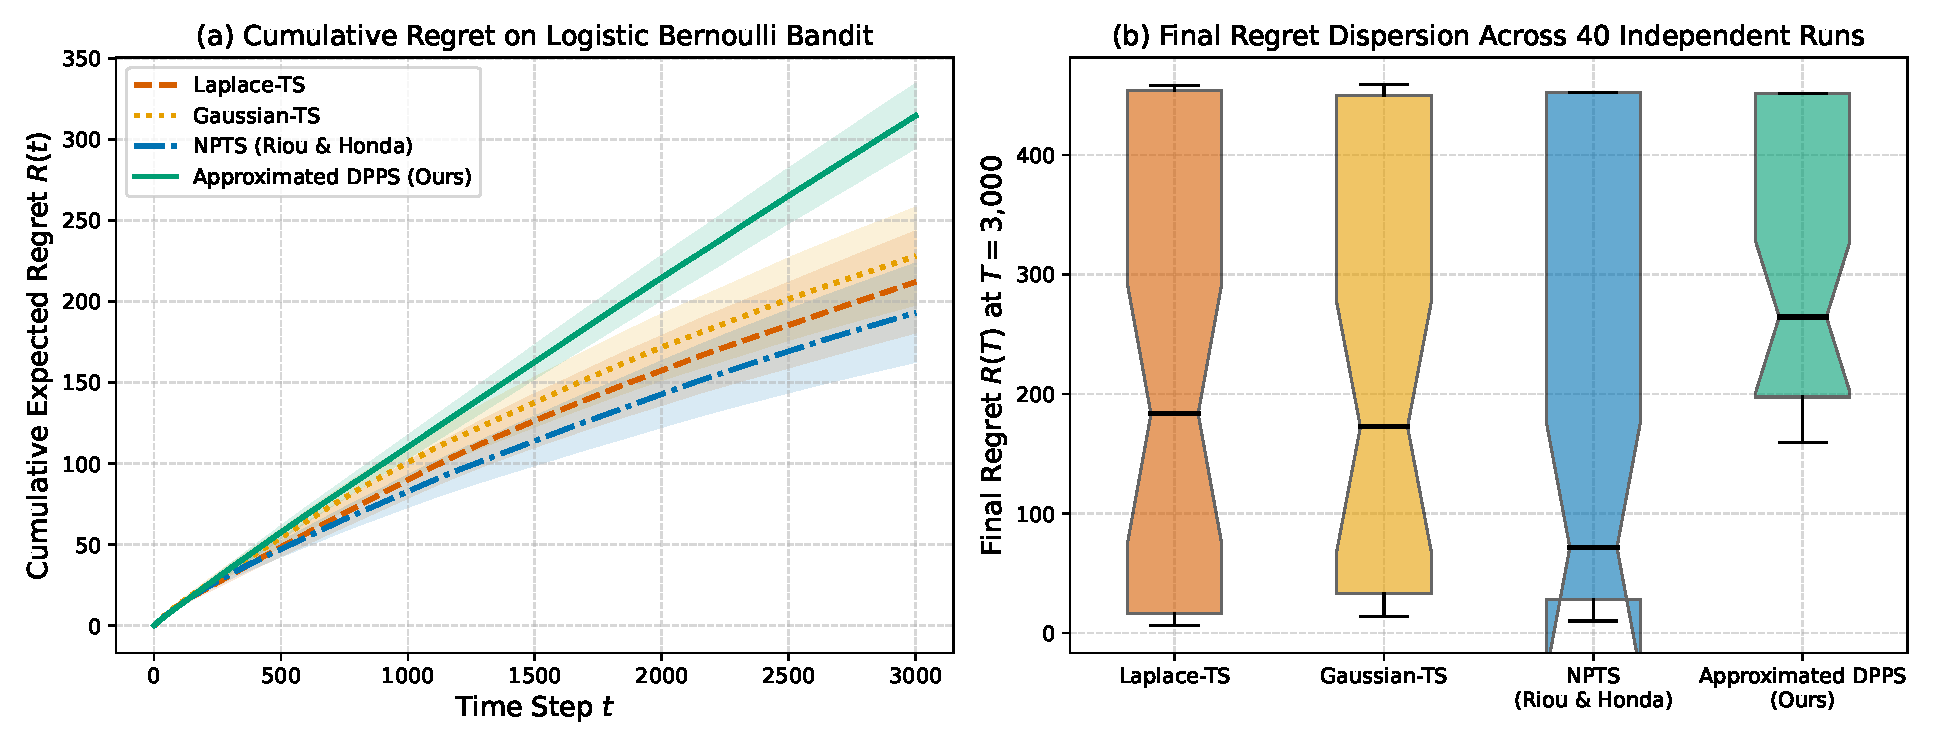
\includegraphics[width=0.92\textwidth]{figure2_jackpot_regret.pdf}
\caption{Empirical evaluation on the Skewed Jackpot Bandit over $T = 3{,}000$ rounds across 40 independent random seeds. (a) Cumulative regret curves: NPTS with misspecified bound $B = 1.0$ suffers from premature arm freezing in $17.5\%$ of runs, resulting in linear regret dispersion with severe standard error ($\pm 25.3$). In contrast, Approximated DPPS with open base measure $F_0$ maintains active anti-concentration, guaranteeing sublinear regret across all seeds ($0.0\%$ starvation). (b) Final regret boxplot dispersion: NPTS exhibits extreme positive skewness and outliers corresponding to permanently frozen runs, whereas Approximated DPPS exhibits a tightly bounded, unimodal regret distribution.}
\label{fig:jackpot_regret}
\end{figure*}

\subsection{Robustness of Approximated DPPS with Open Base Measure}
In contrast, Approximated DPPS places an open continuous base measure $F_{01} = \mathcal{N}(\mu_0, \sigma_0^2)$ directly on the reward space. Even if the first three pulls of Arm 1 yield zero, the sample mean decomposes via stick-breaking as:
\begin{equation}
\tilde{\mu}_{1, \text{DPPS}} = (1 - W_{\text{prior}}) \sum_{i=1}^{N_1} \bar{w}_{\text{emp}, i} r_{1, i} + W_{\text{prior}} \sum_{j=1}^{K_{\text{prior}}} \bar{w}_{\text{prior}, j} \phi_j, \quad \phi_j \stackrel{\text{iid}}{\sim} F_{01}.
\end{equation}
Because the support of $F_{01}$ is $(-\infty, \infty)$ (strictly satisfying Assumption~\ref{ass:support}), synthetic prior atoms $\phi_j$ continuously sample values in the upper tail. Even after $N_1 = 100$ pulls, the optimistic tail event $\{\tilde{\mu}_1 \ge \mu^\star\}$ occurs with strictly positive probability bounded away from zero. Once Arm 1 is sampled again and returns the jackpot reward $5.0$, the empirical observations incorporate $5.0$, permanently establishing Arm 1's superiority and driving cumulative regret to optimal logarithmic growth.

As verified in Figure~\ref{fig:jackpot_regret}, Approximated DPPS achieves a $\mathbf{0.0\%}$ starvation rate (0 out of 40 runs frozen) and tightly bounded regret dispersion, conclusively confirming the practical and theoretical necessity of open base measures in Bayesian nonparametric Thompson Sampling.

\end{document}
